%%%% ijcai15.tex

\typeout{IJCAI-15 Instructions for Authors}

% These are the instructions for authors for IJCAI-15.
% They are the same as the ones for IJCAI-11 with superficical wording
%   changes only.

\documentclass{article}
% The file ijcai15.sty is the style file for IJCAI-15 (same as ijcai07.sty).
\usepackage{ijcai15}

% use Times
\usepackage{times}
% For figures
\usepackage{graphicx} % more modern
%\usepackage{epsfig} % less modern
\usepackage{subfigure} 

% For citations
\usepackage{natbib}

% For algorithms
\usepackage{algorithm}
\usepackage{algorithmic}
\usepackage{hyperref}

\usepackage{amsthm}
\usepackage{amsmath}
\usepackage{amssymb}
%\usepackage{algorithm}
%\usepackage{algorithmic}
%\usepackage{subfig}
%
%\usepackage{bbm}

\newcounter{thm_counter}
\newcounter{lem_counter}
\newcounter{pro_counter}
%\newcounter{cor_counter}
\newcounter{ass_counter}

\newtheorem{theorem}[thm_counter]{Theorem}%[section]
\newtheorem{proposition}[pro_counter]{Proposition}%[section]
\newtheorem{lemma}[lem_counter]{Lemma}%[Lemma]
%\newtheorem{corollary}[cor_counter]{Corollary}
\newtheorem{assumption}[ass_counter]{Assumption}
\newtheorem{remark}[ass_counter]{Remark}

\begin{document}


%\setcounter{chapter}{2} % If you are doing your chapter as chapter one,
%\setcounter{section}{3} % comment these two lines out.

\title{\Large Minimum Volume Multi-Task Learning}
%\author{Bo Liu\thanks{School of Computer Science, University of Massachusetts, boliu@cs.umass.edu}
%\and
%Ji Liu\thanks{Department of Computer Sciences, University of Rochester, jliu@cs.rochester.edu}
%\and
%Hao Men\thanks{Bloomberg L.P. R\&D, New York City, NY, 10022, hao.men@gmail.com}
%\and
%Sridhar Mahadevan\thanks{School of Computer Science, University of Massachusetts, mahadeva@cs.umass.edu}
%\and
%Yong Ge\thanks{Department of Computer Science, University of North Carolina at Charlotte, yong.ge@uncc.edu}
%\and
%Deguang Kong\thanks{Samsung Research America, San Jose, CA, 95134, doogkong@gmail.com}
%}
\date{}

\maketitle

 
%\pagenumbering{arabic}
%\setcounter{page}{1}%Leave this line commented out.

\begin{abstract} \small\baselineskip=9pt 

Multi-Task Learning (MTL) utilizes the intrinsic relationship among
multiple related tasks to reach better generalization and improved
performance. This paper studies the problem of multiple related
supervised learning tasks with task relatedness in the predictor space.
Given the assumption that the predictor relatedness can be interpreted with a
\emph{low-dimensional shared structure} in the intrinsic space
and a \emph{minimum-volume clusteredness} in the ambient space, the problem
formulations with a low-rank regularizer and a non-convex volume constraint
is introduced to depict the low-dimensional shared structure and ambient space
clusteredness respectively. The objective function is solved via alternating
direction method of multipliers(ADMM), which facilitates distributed computation.
Theoretical analysis is also conducted on the solution properties with error boundary
 analysis. Experimental results proove the effectiveness and efficiency of
this proposed framework.

\end{abstract}



\section{Introduction}

Complex real-world problems can usually be decomposed by multiple related tasks and resolved afterward.
An intuitive approach is to apply single task learning on each task independently,
which leads to obvious drawback of not utilizing task relatedness.
Growing interest in Multi-Task
Learning (MTL) or ``Learning to Learn'' appeared in recent decades, multiple
related tasks are learned simultaneously by extracting appropriate shared information
across tasks. In MTL, multiple tasks are assumed correlated to
each other, consequently learning them simultaneously is expected to
conduct both improved prediction performance and better generalization
capability. Applications fields of multi-task learning include bioinformatics,
computer vision, natural language processing and finance. There are
two major approaches to model relatedness among tasks based on making
task related assumptions in predictor space or feature space.
The first approach is to assume there exists task relatedness in the predictor
space, i.e., the task predictors either share a low-dimensional subspace,
or can be clustered in the predictor space. The second is to model task
relatedness based on the assumption that tasks share a common feature
space instead of assuming task relations in the predictor space \cite{mtl:aso:ando2005framework,mtl:mlj2008:argyriou2008convex}.
These algorithms are referred as ``Multi-Task Feature Learning''
(MTFL). In this paper, research is focused on algorithms of the first kind with assumptions 
on task relatedness in the predictor space. 

There are several important topics in MTL including low-dimensional
shared structure, task clusteredness, regularization, hierarchy and convex formulation, etc. Low-dimensional
shared structure is one of the most critical problems to resolve. Different approaches have been proposed to interpret low-dimensional
task relatedness. In many cases, a low rank assumption is made, and then introduced the trace norm regularization in \cite{ji2009accelerated,mtl:siam2010:pong2010trace}. Another
approach assumes that the MTL models lie in a common low-dimensional
subspace \cite{mtl:icml2009:chen2009convex,mtl:NIPS2012:zhang,mtl:aso:ando2005framework}.
In \cite{mtl:aso:ando2005framework}, related tasks are assumed
to share a latent common basis structure, then this non-convex problem
formulation is solved via alternating structure optimization (ASO),
which belongs to one of alternating optimization technique.
The ASO formulation can also be relaxed to a convex problem in \cite{mtl:icml2009:chen2009convex}. 

Besides the low-dimensional shared structure issue, the second important
issue is  task clusteredness. A large family of algorithms assume
that tasks can be clustered in  task space, as investigated in \cite{cmtl:icml2012:flexiblecluster:zhong2012convex,cmtl:ICML2012:Kumar_690,cmtl:NIPS2008:bach,cmtl:nips2011:zhou2011clustered}.
One approach assumes that all predictors are necessarily close to each other in
 task space, this can either be measured by various distance metrics, or sharing
a common prior in the Bayesian framework \cite{mtl:icml2005:yu2005learning,mtl:nips2005:ica:zhang2006learning}.
Both assumptions, including low-dimensional shared structure and task clusteredness in the ambient space, are common and realistic assumptions widely utilized in MTL research. 
However, few research has been conducted on integrating the low-dimensional shared structure with ambient space clusteredness till present.

This paper introduces research to explore the integration of low-dimensional
shared structure with minimum volume task clusteredness. In real-world
multi-task learning problems, the tasks can usually be composed of
components which share common structure in the low-dimensional intrinsic
space, and clusteredness in high dimensional ambient space. To depict both task clusteredness
and low-dimensional shared structure, the geometric
interpretation of task relatedness is explored, i.e., predictors are
clustered and share latent low-dimensional structure in the predictor
space. Therefore, the minimum volume constraint and low-rank
constraint are introduced to depict the clusteredness and low-dimensional structure
respectively, which are both non-convex and non-smooth. The low rank
constraint is utilized to model the low-dimensional structure of the
latent space embedded in the high-dimensional ambient predictor space.
The minimum volume constraint helps to enforce the clusteredness of
the predictors. To ensure the problem solvable, convex relaxation is
enforced to convert the low rank regularization to trace norm regularization and to convert the minimum volume constraint to the group
norm constraint. The algorithm is well designed to be suitable for parallel
computation in several perspectives. The objective function is developed
to be task-separable by introducing an $l_{2,\infty}$ constraint, and the alternative direction multiplier method
(ADMM) is applied to facilitate parallel computation.

Section 2 covers definitions and notations, backgrounds on matrix volume and ADMM are also given. Section 3 presents motivations, problem formulations
and algorithms. Section 4 conducts theoretical analysis including the theoretical guarantee of the solution and error boundary analysis.
Empirical experimental studies are illustrated in Section 5 to validate the efficacy of the proposed algorithms and conclusions are presented in Section 6.


\section{Background}
Notations in this paper are introduced at the beginning, a brief overview of ADMM is given afterwards, ADMM is adopted as the major solver in this paper.

\subsection{Definitions and Notations}
First of all, the fundamental concepts of this paper is the predictor space, a predictor $p$ is a function
that maps an input vector $x\in X$ to the corresponding
output $y\in Y$. The set $\mathcal{P}$ containing
all $p$ comprises a functional space, termed the predictor hypothesis
space, or predictor space for short. The objective of MTL is to discover predictor $p$ from $\mathcal{P}$, which minimizes the empirical error
of the sample set drawn from a probability distribution $\Xi$. In
a linear predictor space $\mathcal{P}\subseteq\mathbb{R}^{d}$, where
$d$ is the number of features, each predictor function is a point
that lies within the $\mathbb{R}^{d}$ space. 
The loss function of MTL is formulated as \cite{mtl:kdd2011:ChenLY10} 
%
\vskip -0.5cm
\begin{equation}
L(W)=\frac{1}{2T}\sum\limits _{i=1}^{T}{\frac{1}{{n_{i}}}||{Y_{i}}-{X_{i}}W_{i}||_{2}^{2}}
\end{equation}
%
where ${X_i} \in {\mathbb{R}^{{n_i} \times d}},{Y_i} \in {\mathbb{R}^{{n_i} \times 1}}$ are the (data, label) pair for the $i$-th task, and
$W_{i}$ is the $i$-th column of model matrix $W$ as defined above,
$n_{i}$ is the number of samples of the $i$-th task, and there are $T$ tasks.
Other definitions
and notations are summarized in Figure \ref{fig:notationmsma}.
%
\begin{figure}[htb]
%\scriptsize
\center
\vskip 0.01in
\fbox{
\begin{tabular}{p{8cm}}
\begin{itemize}
\item $T$: number of tasks; $d$: number of features
\item For the $i$-th task $(X_i, Y_i)$, $n_i$ is the number of samples. $Y\in\mathbb{R}^{n_{i}\times 1}$ is the label matrix, $X_i \in\mathbb{R}^{n_i\times d}$ is the data matrix.
$N = \sum\nolimits_{i = 1}^T {{n_i}} $ is the total number of samples.
\item $W\in\mathbb{R}^{d\times T}$: the predictor matrix. We use $W_{i}:=W_{(:,i)}\in\mathbb{R}^{d\times 1}$ to represent the predictor parameter for the $i$-th task. Also, for any predictor component matrix $U,V$, ${(\cdot)_i} = {(\cdot)_{(:,i)}}$ stands for the $i$-th column of the matrix for $U,V\in\mathbb{R}^{d\times T}$.
\item Frobenius norm: $||A||_{F}^{2}=\sum_{i,j}|a_{ij}|^{2}$
\item Group norm: Let $X\in R^{m\times n},$ Given two vector norms $||\cdot||_{r}$
and $||\cdot||_{p}$, the group norm $||X||_{r,p}$ is defined as
%
\[
||X||_{r,p}=||(||X_{1}||_{r},||X_{2}||_{r},\cdots,||X_{n}||_{r})^{T}||_{p}
\]
%
namely, $||X||_{r,p}$ is to apply $||\cdot||_{r}$ to each column
of $X$, and to apply $||\cdot||_{p}$ to the resulting vector.
\item Trace norm $||X|{|_{*}}$ is the sum of all the singular values of
$X$, $||X|{|_*} = \sum\nolimits_i {{\sigma _i}} $.
\item $\left\langle {X,Y} \right\rangle  = {\rm{Trace}}({X^T}Y),\:X,Y \in {\mathbb{R}^{d \times T}}$
\item ${\rm Vol}(S)$: volume of a matrix $S\in R^{m\times n}$, with non-zero
singular values $\sigma_{1},\sigma_{2},\cdots,\sigma_{t}$, and ${\rm Vol}(S)=0$ if $t=0$, otherwise ${\rm Vol}(S)=\prod_{i=1}^{t}\sigma_{i}$%
%\item \textbf{SVT}$(X,\alpha)$ is the singular value thresholding operator, and \textbf{CC}$X,\beta$ is the column-wise group norm constraint operator, which are defined in the Appendix due to space limitations.
\end{itemize}
\end{tabular}}
%\hline \vskip 0.01in
\caption{Notation used in this paper.}
\label{fig:notationmsma}
\end{figure}
%
%
%\vskip -1cm
\subsection{ADMM}

ADMM is an approximation of the dual ascent approach by applying Douglas-Rachford
operator splitting to the dual problem with Augmented Lagrangian
multipliers. 
%%%Dual decomposition \cite{boyd2009convex}, also termed as dual ascent, is an
%%%extensively studied method for a wide range of constrained convex
%%%optimization problems since the dual decomposition formulation allows
%%%for parallel computation if the loss function is separable. Augmented
%%%Lagrangian Multiplier (ALM) is a class of algorithms that add a quadratic
%%%distance metric function to the regular Lagrangian method to better handle
%%%the equality constraints. One limitation of ALM is that it does not
%%%allow dual decomposition due to the cross product involved in the
%%%quadratic distance generating function; To overcome this drawback,
%%%ADMM is proposed which applies Douglas-Rachford operator splitting
%%%method to allow for dual decomposition. ADMM is especially suitable
%%%for convex optimization problems with multiple regularizers and multiple
%%%non-smooth objective functions. ADMM is a special case of Douglas-Rachford
%%%operator splitting method and Peaceman-Rachford operator splitting
%%%method. 
A typical application of ADMM is the following problem with separable
objective functions (w.r.t variables) and coupled constraint, 
%
\begin{equation}
{\min_{x,y}}f(x)+g(y),\quad{\rm {s.t.}}\:Ax+By=c
\end{equation}
%
The Augmented Lagrangian  Multiplier (ALM) formulation $\Psi(x,y,\lambda)$ is as
follows
% 
\begin{eqnarray}
\nonumber
\Psi (x,y,\lambda ) &=& f(x) + g(y) +  \left\langle {\lambda ,Ax + By - c} \right\rangle \\
& & + \frac{\rho }{2}||Ax + By - c||_2^2
\end{eqnarray}
%
ADMM solves the problem by computing the following update at each iteration, 
\begin{equation}
\begin{array}{l}
{x^{k + 1}} = \arg \mathop {\min }\limits_x f(x) +  \left\langle {\lambda ,Ax} \right\rangle  + \frac{\rho }{2}||Ax + B{y^k} - c||_2^2\\
{y^{k + 1}} = \arg \mathop {\min }\limits_y g(y) +  \left\langle {\lambda ,By} \right\rangle  + \frac{\rho }{2}||A{x^{k+1}} + By - c||_2^2\\
{\lambda ^{k + 1}} = {\lambda ^k} + \rho (A{x^{k + 1}} + B{y^{k + 1}} - c)
\end{array}
\end{equation}


\section{Problem Formulations and Algorithms}

In this section, different problem formulations have been introduced, then propose the corresponding algorithms. The
first formulation assumes that the predictor satisfies both the task clusteredness
and the low-dimensional shared structure. The second problem formulation
assumes that the predictor is a sum of two components which satisfy
the task clusteredness and the low-dimensional relatedness, respectively.
ADMM is utilized as the inner solver of the algorithms.
It is noted that both problem formulations
can  be solved through accelerated gradient \cite{ji2009accelerated},
and using ADMM facilitates large scale parallel computation.


\subsection{Task Relatedness: Low-dimensional Shared Structure and Euclidean
Clusteredness}


This section explains the motivation to apply the methods proposed
in this paper. It is assumed that multi-task model includes
both the low-dimensional shared structure and the (ambient space) clusteredness
structure. The low-dimensional shared structure and clusteredness
can be considered as two geometrical properties of task relatedness
demonstrated in \emph{low-dimensional  intrinsic space}
and \emph{high-dimensional Euclidean ambient space}, respectively.
One common geometrical interpretation of task relatedness is that
the predictor space is a low-dimensional embedding of the ambient
$\mathbb{R}^{d}$ space, which is widely explored in previous MTL
research \cite{cmtl:nips2011:zhou2011clustered,mtl:aso:ando2005framework}.
The low-dimensional shared structure could either be a low-dimensional
manifold \cite{mtl:nips2010:manifold:agarwal2010learning}, a low-rank
structure \cite{ji2009accelerated}, or a shared linear subspace \cite{mtl:aso:ando2005framework}.
The low-dimensional structure in the predictor space is often captured
by either trace norm regularization, or by alternating structure optimization
(ASO) \cite{mtl:aso:ando2005framework}. 

Another common assumption is that tasks are clustered, which is also a geometrical interpretation of task relatedness.
Different from the low-dimensional structure sharing assumption, predictor
clusteredness assumes that the predictors are not far away from each
other in the Euclidean predictor space. One intuitive idea of depicting
this ``predictor closeness/clusteredness'' is to minimize the volume
of the convex hull containing all these predictors. However, it is not
to resolve due to its non-convexity. 
An alternative is to minimize the volume of the ball that contains
the convex hull. To this end, instead of enforcing the non-convex constraint
$V(W)\leq\nu$, controlling the radius of the minimum $l_{2}$
ball containing all the predictors, wherein the centroid is $C$,
and the radius $r$ of the $l_{2}$ ball is $r = \mathop {\max }\limits_i ||{W_i} - C|{|_2}$,
this is equivalent to the group norm formulation of $\|W-C\mathbf{1}^{T}\|_{2,\infty}\leq r$,
where $\mathbf{1} \in \mathbb{R}^{T \times 1}$ with all entries
equal to $1$.  In the case of a single centroid, the Euclidean
mean can be applied to approximate this centroid $C$, i.e., 
$
C \approx W{\bf{1}}/T.
$
 Then the constraint is 
\begin{equation}
\|W-C\mathbf{1}^{T}\|_{2,\infty}\approx\|WD\|_{2,\infty}\leq r,
\end{equation}
where $D=(I-\boldsymbol{11}^{T}/T)$. Note that $D$ is both symmetric and idem-potent, namely, $D=D^{T},D^{2}=D$,
rank($D$)=$T-1$.  


\subsection{Problem Formulation 1}

Given the problem formulation where the model $W$ is assumed to be both low-dimensional and clustered.
To depict the low-dimensional latent space structure, low-rank regularization ${\rm {rank}}(W)$
is introduced. On the other hand, a minimum volume constraint is introduced to enforce the predictors to be clustered together.
Therefore the problem can be formulated as follows
\begin{equation}
\mathop {\min }\limits_W L(W) + \alpha {\rm{rank}}(W),\quad{\rm{s.t.}}\:{\rm{Vol}}(W) \le v
\label{eq:nonconvex1}
\end{equation}
where the regularizer $\alpha{\rm {rank}}(W)$ and the constraint
${\rm {Vol(}}W{\rm {)}}\le v$ are both non-convex and non-smooth.
%Using the singular value representation of ${\rm {Vol(}}W{\rm {)}}=\Pi_{i}{\sigma_{i}}(W)$,
%where $\sigma_{i}$ is the $i$-th singular value of $W$, we have
%an equivalent representation via the singular values of $W$
%\begin{equation}
%\begin{array}{l}
%\mathop {\min }\limits_W \frac{1}{{2T}}\sum\limits_{i = 1}^T {\frac{1}{{{n_i}}}||{Y_i} - {X_i}{W_i}||_F^2}  + \alpha {\rm{NNZ}}({\sigma _i}(W)),\\
%{\rm{s}}.{\rm{t}}\:\mathop \Pi \limits_i {\sigma _i}(W) \le v
%\end{array}
%\label{eq:nonconvex1-1}
%\end{equation}
Next to consider the convex relaxations.
The rank norm regularization is relaxed to the trace norm regularization \cite{ji2009accelerated},
and the minimum volume constraint is relaxed as discussed
above. Thus (\ref{eq:nonconvex1}) is relaxed as
%
\begin{equation}
{\mathop {\min }\limits_W L(W) + \alpha ||W|{|_*},\quad{\rm{s.t.}}\:||WD|{|_{2,\infty }} \le r}
\label{eq:nc1-2}
\end{equation}
%
Now the problem can be formulated as a convex smooth objective function
with a convex non-smooth trace norm penalty and a convex non-smooth
group norm constraint. 

\subsection{Algorithm 1}

Algorithm 1 aims to solve the objective function of Equation (\ref{eq:nc1-2}).
The ALM formulation is 
\begin{eqnarray}
\nonumber
&& \Psi (W,S,U,V,{\lambda _1},{\lambda _2},{\lambda _3})\\
\nonumber
&=& L(W)+\alpha\|U\|_{*}+ \left\langle {{\lambda _1},S - VD} \right\rangle  + \frac{{{\rho _1}}}{2}||S - VD|{|^2}\\
\nonumber
&& +\left\langle {{\lambda_{2}},U-W}\right\rangle +\frac{{\rho_{2}}}{2}||U-W||^{2}\\
\nonumber
&& +\left\langle {{\lambda_{3}},V-W}\right\rangle +\frac{{\rho_{3}}}{2}||V-W||^{2}
\quad{\rm s.t.}\:||S|{|_{2,\infty}\leq r}
\label{eq:nc1-admm}
\end{eqnarray}
%
The update rule is
%
\begin{eqnarray}
\label{eq:admm1}
\nonumber
{S^{k+1}} &=& {\bf{CC}}({V^k}D{\rm{ - }}\frac{{\lambda ^k_1}}{{{\rho _1}}},r)\\
\nonumber
{U^{k+1}} &=& {\bf{SVT}}({W^k}{\rm{ - }}\frac{{\lambda ^k_2}}{{{\rho _2}}},\frac{\alpha }{{{\rho _2}}})\\
\nonumber
{V^{k+1}} &=& \left[ {{\lambda ^k_1}D - \lambda ^k_3 + {\rho _1}{S^{k + 1}}D + {\rho _3}{W^k}} \right] \cdot \\
&&{\left({{\rho_{1}}{D^{2}}+{\rho_{3}}{\rm {I}}}\right)^{-1}}
\end{eqnarray}
For each task, $W^{k+1}_{i}$ is updated as
%
\begin{equation}
\begin{array}{l}
W_i^{k + 1} = {(\frac{1}{{T{n_i}}}{X_i}^T{X_i} + ({\rho _2} + {\rho _3})I)^{ - 1}} \cdot \\
\left(\frac{1}{{T{n_i}}}{X_i}^T{Y_i} + {\lambda^k _{2,i}} + {\lambda^k _{3,i}} + {\rho _2}U_i^{k + 1} + {\rho _3}V_i^{k + 1}\right)
\end{array}
\label{eq:nc1-w}
\end{equation}
%
where \textbf{SVT} is the singular value thresholding operator and \textbf{CC} is the column-wise group norm constraint operator, which are both detailed in the Appendix.
To cache the factorization result, the matrix inversion lemma can be used,
which is described in detail in the supplementary material due to space considerations. 
${\lambda^{k + 1}_{1}}, {\lambda^{k + 1}_{2}}, {\lambda^{k + 1}_{3}}$ are updated as
\begin{equation}
\begin{array}{*{20}{l}}
{\lambda _{_1}^{k + 1} = \lambda _{_1}^k + {\rho _1}({S^{k + 1}} - {V^{k + 1}}D)}\\
{\lambda _{_2}^{k + 1} = \lambda _{_2}^k + {\rho _2}({U^{k + 1}} - {W^{k + 1}})}\\
{\lambda _3^{k + 1} = \lambda _3^k + {\rho _3}({V^{k + 1}} - {W^{k + 1}})}
\end{array}
\label{eq:lambda1}
\end{equation}
%
The illustration is shown in Figure \ref{fig:mtl1}, where model $W$ is assumed to be both low-rank and all the predictors stay within the $l_2$ ball with radius $r$.
%
\begin{figure}[!htb]
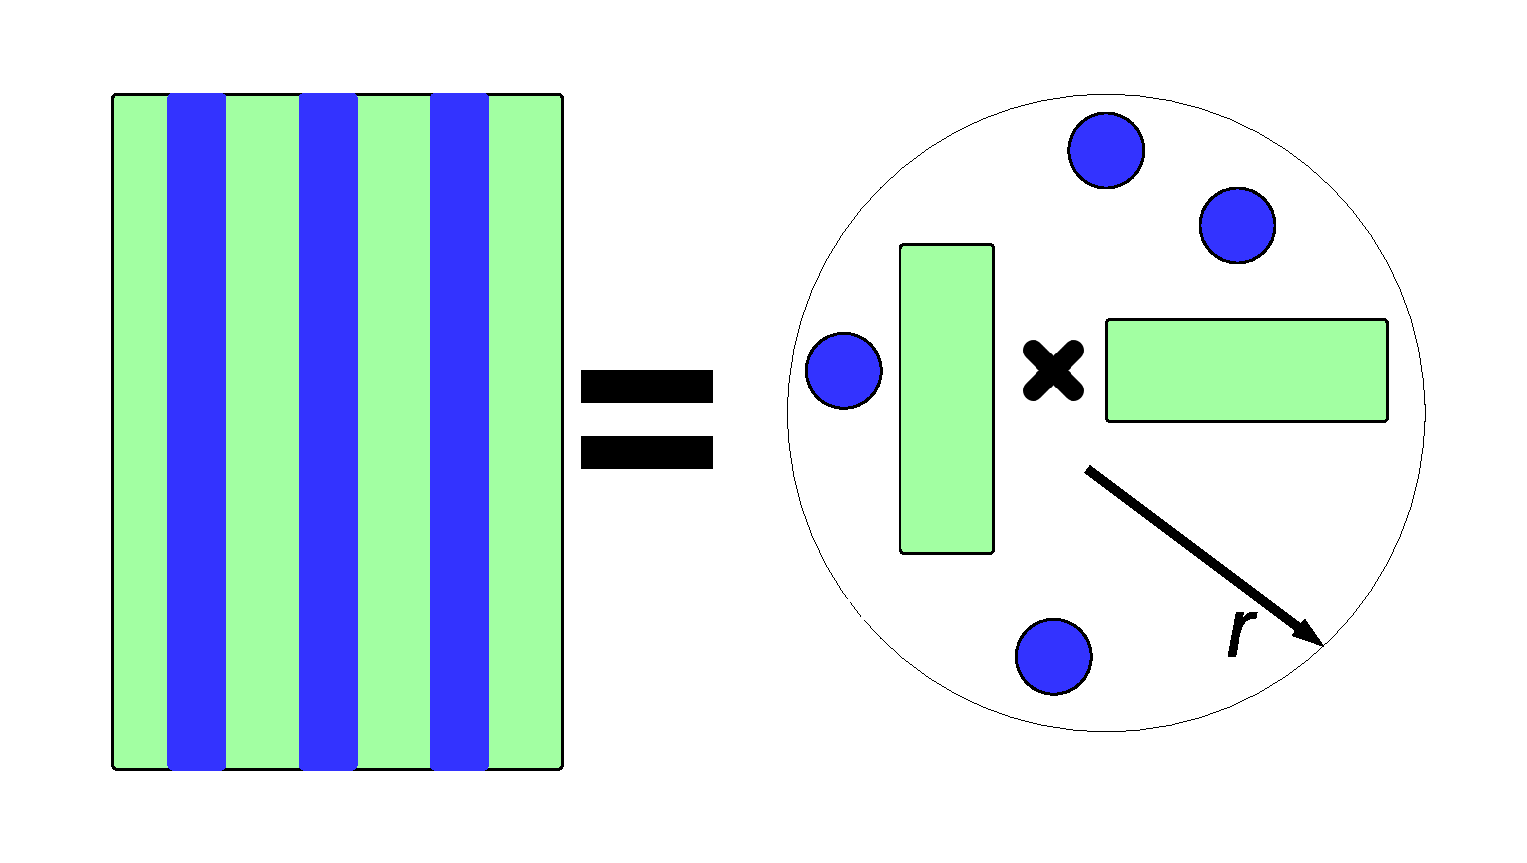
\includegraphics[width= .5\textwidth, height=1.1in]{figures/mtl1.pdf}
\caption{Illustration of Problem Formulation 1}
\label{fig:mtl1}
\end{figure}
%
%
\begin{algorithm}
\label{alg:mvmtl1}
\caption{Minimum Volume MTL 1 (MVMTL1) }
\textbf{INPUT}: $\{X,Y\}=\{X_{i,}Y_{i}\}_{i=1}^{T}$ for MTL learning\\
\textbf{OUTPUT}: $W$ 
\begin{algorithmic}[1]
\REPEAT
\STATE Update ${S^{k+1}},{U^{k+1}},{V^{k+1}},{W^{k+1}}$ via (\ref{eq:admm1}, \ref{eq:nc1-w})
\STATE Update $\lambda^{k+1}_{1},\lambda^{k+1}_{2},\lambda^{k+1}_{3}$ via (\ref{eq:lambda1})
\UNTIL Some stopping criteria is met;
\end{algorithmic}
\end{algorithm}

\subsection{Problem Formulation 2}

Another problem formulation assumes that the model $W$ is a sum of a low-dimensional shared structure $U$ and a Euclidean clustered structure $V$. To this end, the problem formulation is presented as follows,
%
\begin{equation}
\mathop {\min }\limits_{U,V} L(U+V)
 + \alpha {\rm{rank}}(U),\quad{\rm{s.t.}}\:{\rm{Vol}}(V) \le v,
\label{eq:nonconvex2}
\end{equation}
which can be relaxed as
\begin{equation}
\mathop {\min }\limits_{U,V} L(U+V)  + \alpha ||U|{|_*},\quad{\rm{s.t.}}\:||VD|{|_{2,\infty }} \le  r
\label{eq:nc2-2}
\end{equation}
The illustration can be seen in Figure \ref{fig:mtl2}, wherein the model $W$ is decomposed to a low-rank component $U$ and a group norm constrained component $V$.
\begin{figure}[h]
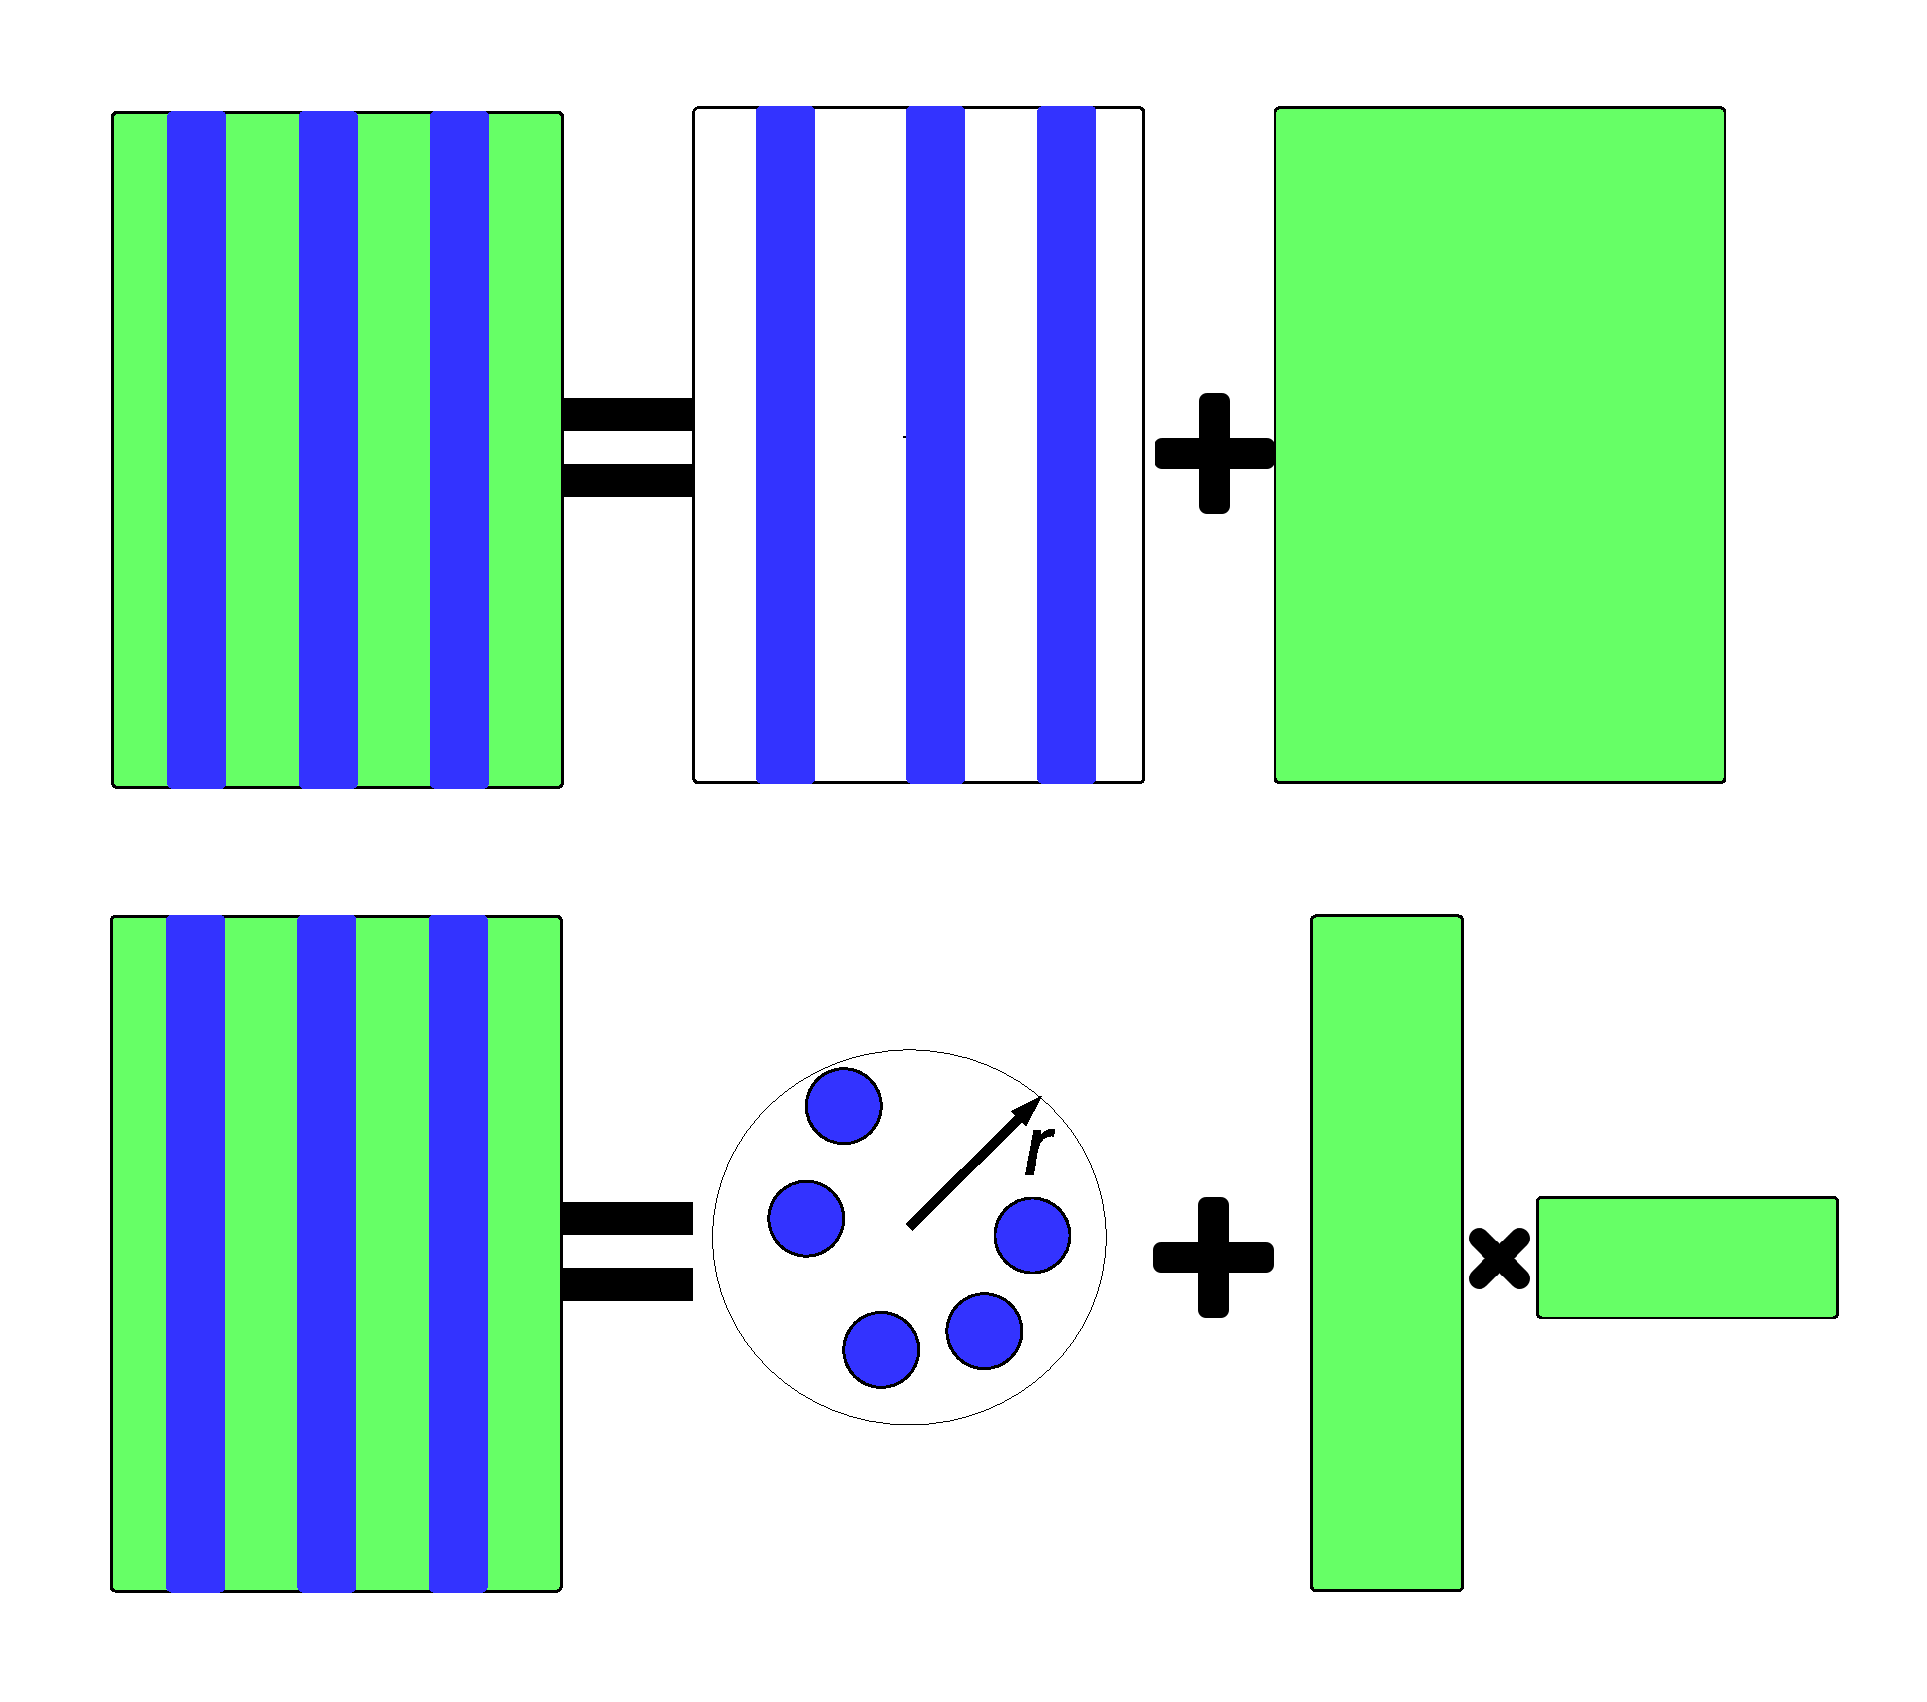
\includegraphics[width= .5\textwidth, height=1.3in]{figures/mtl2.pdf}
\caption{Illustration of Problem Formulation 2}
\label{fig:mtl2}
\end{figure}

\subsection{Algorithm 2}

The loss function of Algorithm 2 is Equation (\ref{eq:nc2-2}). The ALM formulation is 
%
\begin{eqnarray}
\nonumber
&&{\Psi (W,S,U,V,{\lambda _1},{\lambda _2})}\\
\nonumber
&=& L(W)+\alpha\|U\|_{*}
+\left\langle {{\lambda_{1}},S-VD}\right\rangle  +\frac{{\rho_{1}}}{2}||S-VD|{|^{2}}\\
\nonumber
&& +\left\langle {{\lambda_{2}},U+V-W}\right\rangle +\frac{{\rho_{2}}}{2}||U+V-W|{|^{2}},\\
&& \:{\rm{s.t.}}\:||S|{|_{2,\infty}\leq r}
\label{eq:nc2-admm}
\end{eqnarray}
The update rule is
%
\begin{eqnarray}
\nonumber
{S^{k+1}} &=& {\rm {\textbf{CC}}}({V^k}D-\frac{{\lambda^k_{1}}}{{\rho_{1}}},r)\\
\nonumber
{U^{k+1}} &=& {\rm {\textbf{SVT}}}({W^{k}}-{V^{k}}{\rm {-}}\frac{{\lambda^k_{2}}}{{\rho_{2}}},\frac{\alpha}{{\rho_{2}}})\\
\nonumber
{V^{k+1}} &=& \left[{{\lambda^k_{1}}D-{\lambda^k_{2}}+{\rho_{1}}{S^{k+1}}D+{\rho_{2}}({W^{k}}-{U^{k+1}})}\right]\cdot \\
&&{\left({{\rho_{1}}{D^{2}}+{\rho_{2}}{\rm {I}}}\right)^{-1}}
\label{eq:admm2}
\end{eqnarray}
For each task, $W^{k + 1}_{i}$ is updated as
\begin{eqnarray}
\nonumber
W_{i}^{k+1}&=&{(\frac{1}{{T{n_{i}}}}X_{^{i}}^{T}{X_{i}}+{\rho_{2}}I)^{-1}}\cdot\\
&&\left(\frac{1}{{T{n_{i}}}}X_{^{i}}^{T}{Y_{i}}+{\lambda^k_{2,i}}+{\rho_{2}}(U_{i}^{k+1}+V_{i}^{k+1})\right)
\label{eq:nc2-w}
\end{eqnarray}
And ${\lambda^{k + 1}_{1}}, {\lambda^{k + 1}_{2}}$ are updated as
\begin{equation}
\begin{array}{*{20}{l}}
{\lambda _{_1}^{k + 1} = \lambda _{_1}^k + {\rho _1}({S^{k + 1}} - {V^{k + 1}}D)}\\
{\lambda _2^{k + 1} = \lambda _{_2}^k + {\rho _2}({U^{k + 1}} + {V^{k + 1}} - {W^{k + 1}})}
\end{array}
\label{eq:lambda2}
\end{equation}
%
%
\begin{algorithm}
\label{alg:mvmtl2}
\caption{Minimum Volume MTL 2 (MVMTL2) }
\textbf{INPUT}: $\{X,Y\}=\{X_{i,}Y_{i}\}_{i=1}^{T}$ for MTL learning\\
\textbf{OUTPUT}: $W=U+V$
\begin{algorithmic}[1]
\REPEAT
\STATE Update ${S^{k+1}},{U^{k+1}},{V^{k+1}},{W^{k+1}}$ via (\ref{eq:admm2},\ref{eq:nc2-w})
\STATE Update $\lambda^{k+1}_{1},\lambda^{k+1}_{2}$ via (\ref{eq:lambda2}) 
\UNTIL Some stopping criteria is met;
\end{algorithmic}
\end{algorithm}

%\subsection{Clustered MVMTL}
%
%Instead of assuming the data are centred around its column mean, next problem assume there exists a point $c_{1}$
%in the predictor space which minimizes the max of $l_{2}$ distance
%of all the predictors with respect to (w.r.t.) $c_{1}$. Therefore the
%objective function is reformulated as 
%\begin{equation}
%{\mathop {\min }\limits_{U,V,{c_1}} L(U+V),\quad{\rm{s.t.}}\:||V - {c_1}{1^T}|{|_{2,\infty }} \le r}
%\label{eq:probform:c1}
%\end{equation}
%Note this formulation considers the centroid $c_{1}$ as a variable,
%and in the Euclidean space $c_{1}$ is expected to be the mean of columns
%of $V$.
%
%The aforementioned MTL framework can be easily extended to clustered
%multi-task learning problems. If there are $k$ task clusters such that 
%\begin{equation}
%{\mathop {\min }\limits_{U,V,C} L(U + V) + \alpha ||U|{|_*},\quad{\rm{s.t.}}\:||V - C{I_c}|{|_{2,\infty }} \le r}
%\label{eq:clusterMTL}
%\end{equation}
%Where $C=[\begin{array}{cccc}
%{c_{1}} & {c_{2}} & \cdots & {c_{k}}\end{array}],$ and $c_{i}$ is the centroid of the $i$-th task cluster and ${I_{c}}\in{\mathbb{R}^{k\times T}}$ is the cluster indicator
%function defined as 
%\begin{equation}
%{I_c}[i,j] = \left\{ {\begin{array}{*{20}{c}}
%1&{{\rm{task}}\:j \in {\rm{cluster}}\: i}\\
%0&{{\rm{task}}\:j \notin {\rm{cluster}}\: i}
%\end{array}} \right.
%\end{equation}
%The ALM formulation is
%%
%\begin{eqnarray}
%\nonumber
%&& \Psi (W,S,U,V,{\lambda _1},{\lambda _2})\\
%\nonumber
%&=& L(W) + \alpha ||U|{|_*}\\
%\nonumber
%&&  + \left\langle {{\lambda _1},S - V + C{I_c}} \right\rangle + \frac{{{\rho _1}}}{2}||S - V + C{I_c}|{|^2} \\
%\nonumber
%&& { + \left\langle {{\lambda _2},U + V - W} \right\rangle  + \frac{{{\rho _2}}}{2}||U + V - W|{|^2},}\\
%&& {\:{\rm{s.t.}}\:||S|{|_{2,\infty }} \le r}
%\end{eqnarray}
%%
%The update rule is
%\begin{eqnarray}
%\nonumber
%{S^{k + 1}} &=& {\bf{CC}}({V^k} - {C^k}{I_c},r)\\
%\nonumber
%{U^{k+1}} &=& {\rm {\textbf{SVT}}}({W^{k}}-{V^{k}}{\rm {-}}\frac{{\lambda^k_{2}}}{{\rho_{2}}},\frac{\alpha}{{\rho_{2}}})\\
%\nonumber
%{V^{k + 1}} &=& \frac{1}{{{\rho _1} + {\rho _2}}}\cdot\\
%\nonumber
%&&\left( {{\lambda^k _1} + {\rho _1}{S^{k+1}} + {\rho _1}{C^k}{I_c} - {\lambda^k _2} - {\rho _2}{U^{k+1}} - {\rho _2}{W^k}} \right)\\
%\nonumber
%{C^{k + 1}} &=& \left[ {V^{k+1} - S^{k+1} + \frac{{{\lambda^k _1}}}{{{\rho _1}}}} \right]{I_c ^ + }\\
%&&{\left({{\rho_{1}}{D^{2}}+{\rho_{2}}{\rm {I}}}\right)^{-1}}
%\label{eq:admm3}
%\end{eqnarray}
%$W^{k+1}$ is updated as in Equation (\ref{eq:nc2-w}),and ${\lambda^{k + 1}_{1}}, {\lambda^{k + 1}_{2}}$ are updated as
%\begin{equation}
%\begin{array}{*{20}{l}}
%{\lambda _{_1}^{k + 1} = \lambda _{_1}^k + {\rho _1}({S^{k + 1}} - {V^{k + 1}} + {C^{k + 1}}{I_c})}\\
%{\lambda _2^{k + 1} = \lambda _{_2}^k + {\rho _2}({U^{k + 1}} + {V^{k + 1}} - {W^{k + 1}})}
%\end{array}
%\label{eq:lambda3}
%\end{equation}
%where $I_c^ +  = I_c^T{(I_c^TI_c^T)^{ - 1}}$ is the right pseudo-inverse
%The illustration is shown in Figure \ref{fig:mtl-cluster}.
%\begin{figure}[!htb]
%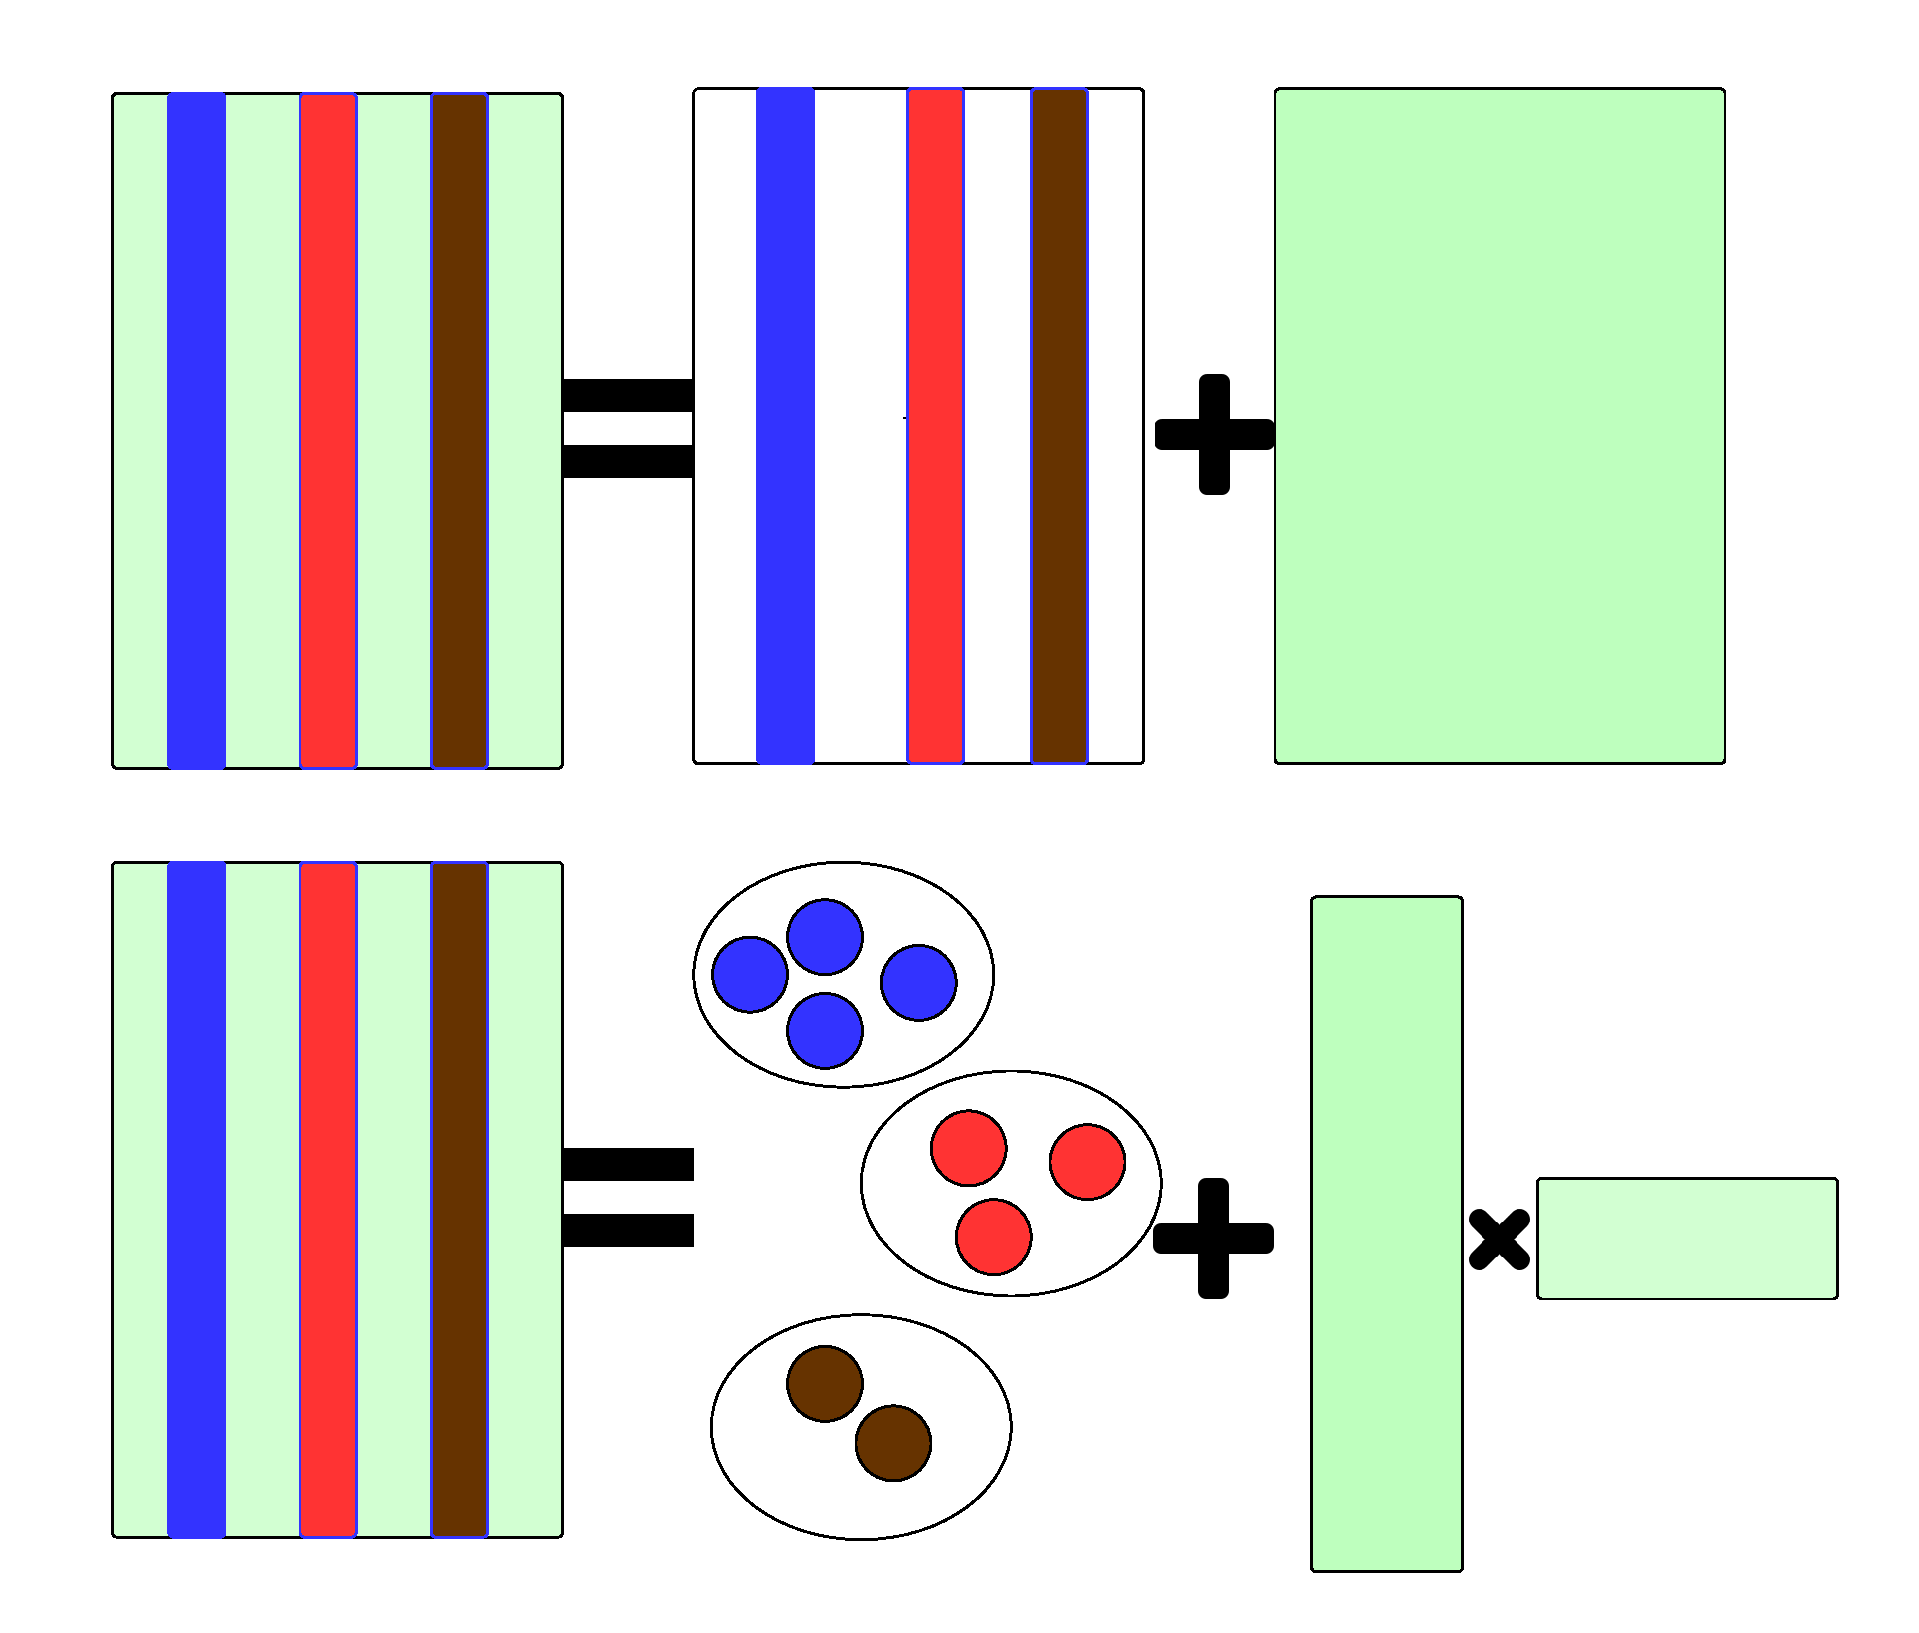
\includegraphics[width= .5\textwidth, height=1.1in]{figures/mtl-cluster.pdf}
%\caption{Illustration of Clustered MTL Formulation}
%\label{fig:mtl-cluster}
%\end{figure}
%%
%


\section{Theoretical Guarantee}

In this section, both theoretical analysis for Algorithm 1 and Algorithm 2 are illustrated. Solution properties are derived and the choice of regularization parameters is presented also.
 Error boundary analysis is also conducted. The theoretical analysis and proof follow the spirit of the analysis in \cite{mtl:kdd2011:ChenZY11}.
Due to space limitation, we will focus on the analysis on Algorithm 2, and the analysis for Algorithm 1 will be elaborated in a longer technical report.

\subsection{Solution Property}

To obtain the solution property, first  convert
the $l_{2,\infty}$ constraint to $l_{2,1}$ regularizers. 
It can be derived that due to the dual norm relation between $l_{2,1}$ norm and $l_{2,\infty}$ norm, for a given radius $r$, there exists a $\beta$
such that the solution of Equation (\ref{eq:nc1-2}) is the solution
of the following formulation,
%
\begin{equation}
\mathop {\min }\limits_W L(W)+\alpha\|W\|_{*}+\beta\|WD\|_{2,1}
\label{eq:nc1-dual}
\end{equation}
And likewise, there is the corresponding formulation of Equation (\ref{eq:nc2-2}) 
%
\begin{equation}
\mathop {\min }\limits_{U,V} L(U+V) +\alpha\|U\|_{*}+\beta\|VD\|_{2,1}
\label{eq:nc2-dual}
\end{equation}
%
Assume the linear predictor for the $i$-th task is formulated as
$
{Y_i} = {f_i}({X_i}) + {\delta _i},
$
where  the stochastic Gaussian noise vector ${\delta _i} \in {\mathbb{R}^{{n_i \times 1}}}$, and each noise entry ${\delta _{ij}} \sim N(0,{\sigma ^2}),\forall j \le {n_i}$. 

\subsection{Error Boundary}

Lemma 1 is presented for the choice of the regularization parameter pair $(\alpha, \beta)$.

\noindent \textbf{Lemma 1}:(Regularization parameters) With high probability
\begin{equation}
{\rm {prob}}\ge{\rm {1-}}\frac{1}{T}\exp\left({-\frac{1}{2}(t-d\log(1+\frac{t}{d}))}\right),
\end{equation}
%
there exists a pair $(\alpha, \beta)$ such that if $\frac{\alpha }{{\sqrt T }},\beta  \ge \frac{{2\sigma }}{N}\sqrt {d + t} $, $t$ is a pre-chosen constant, then the global minimizer ($U^*, V^*$) of problem (\ref{eq:nc2-dual}), and an arbitrary pair $U,V \in {\mathbb{R}^{d \times T}}$, the following holds,
%
\begin{eqnarray}
&& \frac{1}{{2T}}\sum\limits_{i = 1}^T {\frac{1}{{{n_i}}}||{f_i} - {X_i}{{(U^* + V^*)}_i})||_2^2} \\
\nonumber
&\le & \frac{1}{{2T}}\sum\limits_{i = 1}^T {\frac{1}{{{n_i}}}||{f_i} - {X_i}{{(U + V)}_i})||_F^2} \\
\nonumber
&& { + \alpha ||{\rm P}(U - U^*)|{|_*} + \beta ||{\rm Q}(V - V^*)|{|_{2,1}}}
\end{eqnarray}
%
where $(\cdot)_{i}$ denotes the $i$-th column of the matrix. Lemma 1 implies that $(\alpha, \beta)$ should be proportional to $\sqrt{d}$. Given the choice of $(\alpha, \beta)$, we present the error boundary analysis as Theorem 1.

\noindent \textbf{Theorem 1} (Performance of Algorithm 2): Given $(\alpha, \beta)$ chosen following Lemma 1 ,with high probability
\begin{equation}
{\rm {prob}}\ge{\rm {1-}}\frac{1}{T}\exp\left({-\frac{1}{2}(t-d\log(1+\frac{t}{d}))}\right),
\end{equation}
there is a global optimal solution ($U^*, V^*$) of problem (\ref{eq:nc2-2}) satisfying the following,
%\begin{equation}
%\begin{array}{*{20}{l}}
%\begin{array}{l}
%\frac{1}{{2T}}\sum\limits_{i = 1}^T {\frac{1}{{{n_i}}}||{f_i} - {X_i}{{(U^* + V^*)}_i})||_2^2} \\
% \le (1 + \varepsilon )\mathop {\inf }\limits_{U,V} \frac{1}{{2T}}\sum\limits_{i = 1}^T {\frac{1}{{{n_i}}}||{f_i} - {X_i}{{(U + V)}_i})||_2^2} 
%\end{array}\\
%{ + \xi (\varepsilon )\left( {\frac{{{\alpha ^2}}}{{{\kappa^2}(2p)}} + \frac{{{\beta ^2}}}{{{\tau^2}(q)}}} \right)}
%\end{array}
%\end{equation}
\begin{eqnarray}
&&  \frac{1}{{2T}}\sum\limits_{i = 1}^T {\frac{1}{{{n_i}}}||{f_i} - {X_i}{{(U^* + V^*)}_i})||_2^2} \\
\nonumber
&\le& (1 + \varepsilon )\mathop {\inf }\limits_{U,V \in \mathcal{R}( p,q) }  \frac{1}{{2T}}\sum\limits_{i = 1}^T {\frac{1}{{{n_i}}}||{f_i} - {X_i}{{(U + V)}_i})||_2^2} \\
\nonumber
&& { + \xi (\varepsilon )\left( {\frac{{{\alpha ^2}}}{{{\kappa^2}(2p)}} + \frac{{{\beta ^2}}}{{{\tau^2}(q)}}} \right)}
\end{eqnarray}
%
where $t, \varepsilon >0$ are two pre-chosen constants,  constants $p,q$, real functions $\kappa(\cdot), \tau(\cdot)$,  and the restricted set $\mathcal{R}( p,q)$ are all defined in the supplementary material, and $\xi (\varepsilon ) = \frac{{{{(\varepsilon  + 2)}^2}}}{{2\varepsilon }}$. Theorem 1 implies that  error can be decomposed into two terms, where one depends on the formulation of $L(W)$, and the other is controlled by the regularization terms, and both bounds go to zero given the cardinality of the sample set goes to infinity.
Similar analysis can be derived for Algorithm 1, it is not elaborated in detail due to space limitations.


\section{Experiment}

This section evaluates the effectiveness of the proposed two
algorithms. The data set is introduced first, the performance
of the algorithms is measured on two benchmark data sets, the School data and
SARCOS data. The School data is composed of the exam scores of
$15362$ students from $139$ schools, where the students are described
with $21$ features including gender and ethnic group, and each school's
test score is a regression task, so altogether there are $139$ regression
tasks. The SARCOS data is an inverse dynamic prediction problem
for a robot arm with $7$ degrees-of-freedom. There are $48933$ observations
with $28$ entries for each sample, where the initial $21$ entries
are features, and the rest $7$ entries are target values for the
$7$ tasks. Several different measures are used
to ensure fairness in the comparison study. Normalized mean squared error
(nMSE), averaged mean squared error (aMSE), weighted mean squared error (WMSE) and weighted root of sum of squared error (WRSE) are used as evaluation measures, which are defined in the supplementary material.


\subsection{Volume Control Study}

The volume control performance of the
proposed algorithms is presented in this experiment. Set $\alpha=[0,10,20,\cdots, 50, 100, 200, \cdots, 500, 1000]$, and $r=[10, 20, \cdots, 50, 100, 200, \cdots, 500, 1000]$. Figure \ref{fig:v-alpha} shows the results of the volume of the learned model (For MVMTL1, it is $W$, for MVMTL2, it is the clustered component $V$). From the top subfigure of Figure \ref{fig:v-alpha} we can see that for MVMTL1, the radius of the model is affected by both $\alpha$ and $r$, although when $\alpha$ is large (e.g., $\alpha>50$), the impact is reduced.  For MVMTL2, shown in the bottom subfigure of Figure \ref{fig:v-alpha} that $\alpha$ only has impact on the $U$ component, and merely has any impact on the radius of the $V$ model, which is consistent with the theoretical analysis.

The relation between the pre-set radius $r$ and the real radius of the learned model is also evaluated, shown in Figure \ref{fig:v-radius}. From the top subfigure, it is clear to observe that for MVMTL1, a large $\alpha$ helps to reduce the radius of the model, and the radius of the true model often goes beyond the pre-set radius when a small $\alpha$ is used. For MVMTL2, the true radius of the $V$ component is almost strictly consistent with the pre-set radius.  
%
%
\begin{figure}[h]
\centering
\begin{minipage}{1\textwidth}
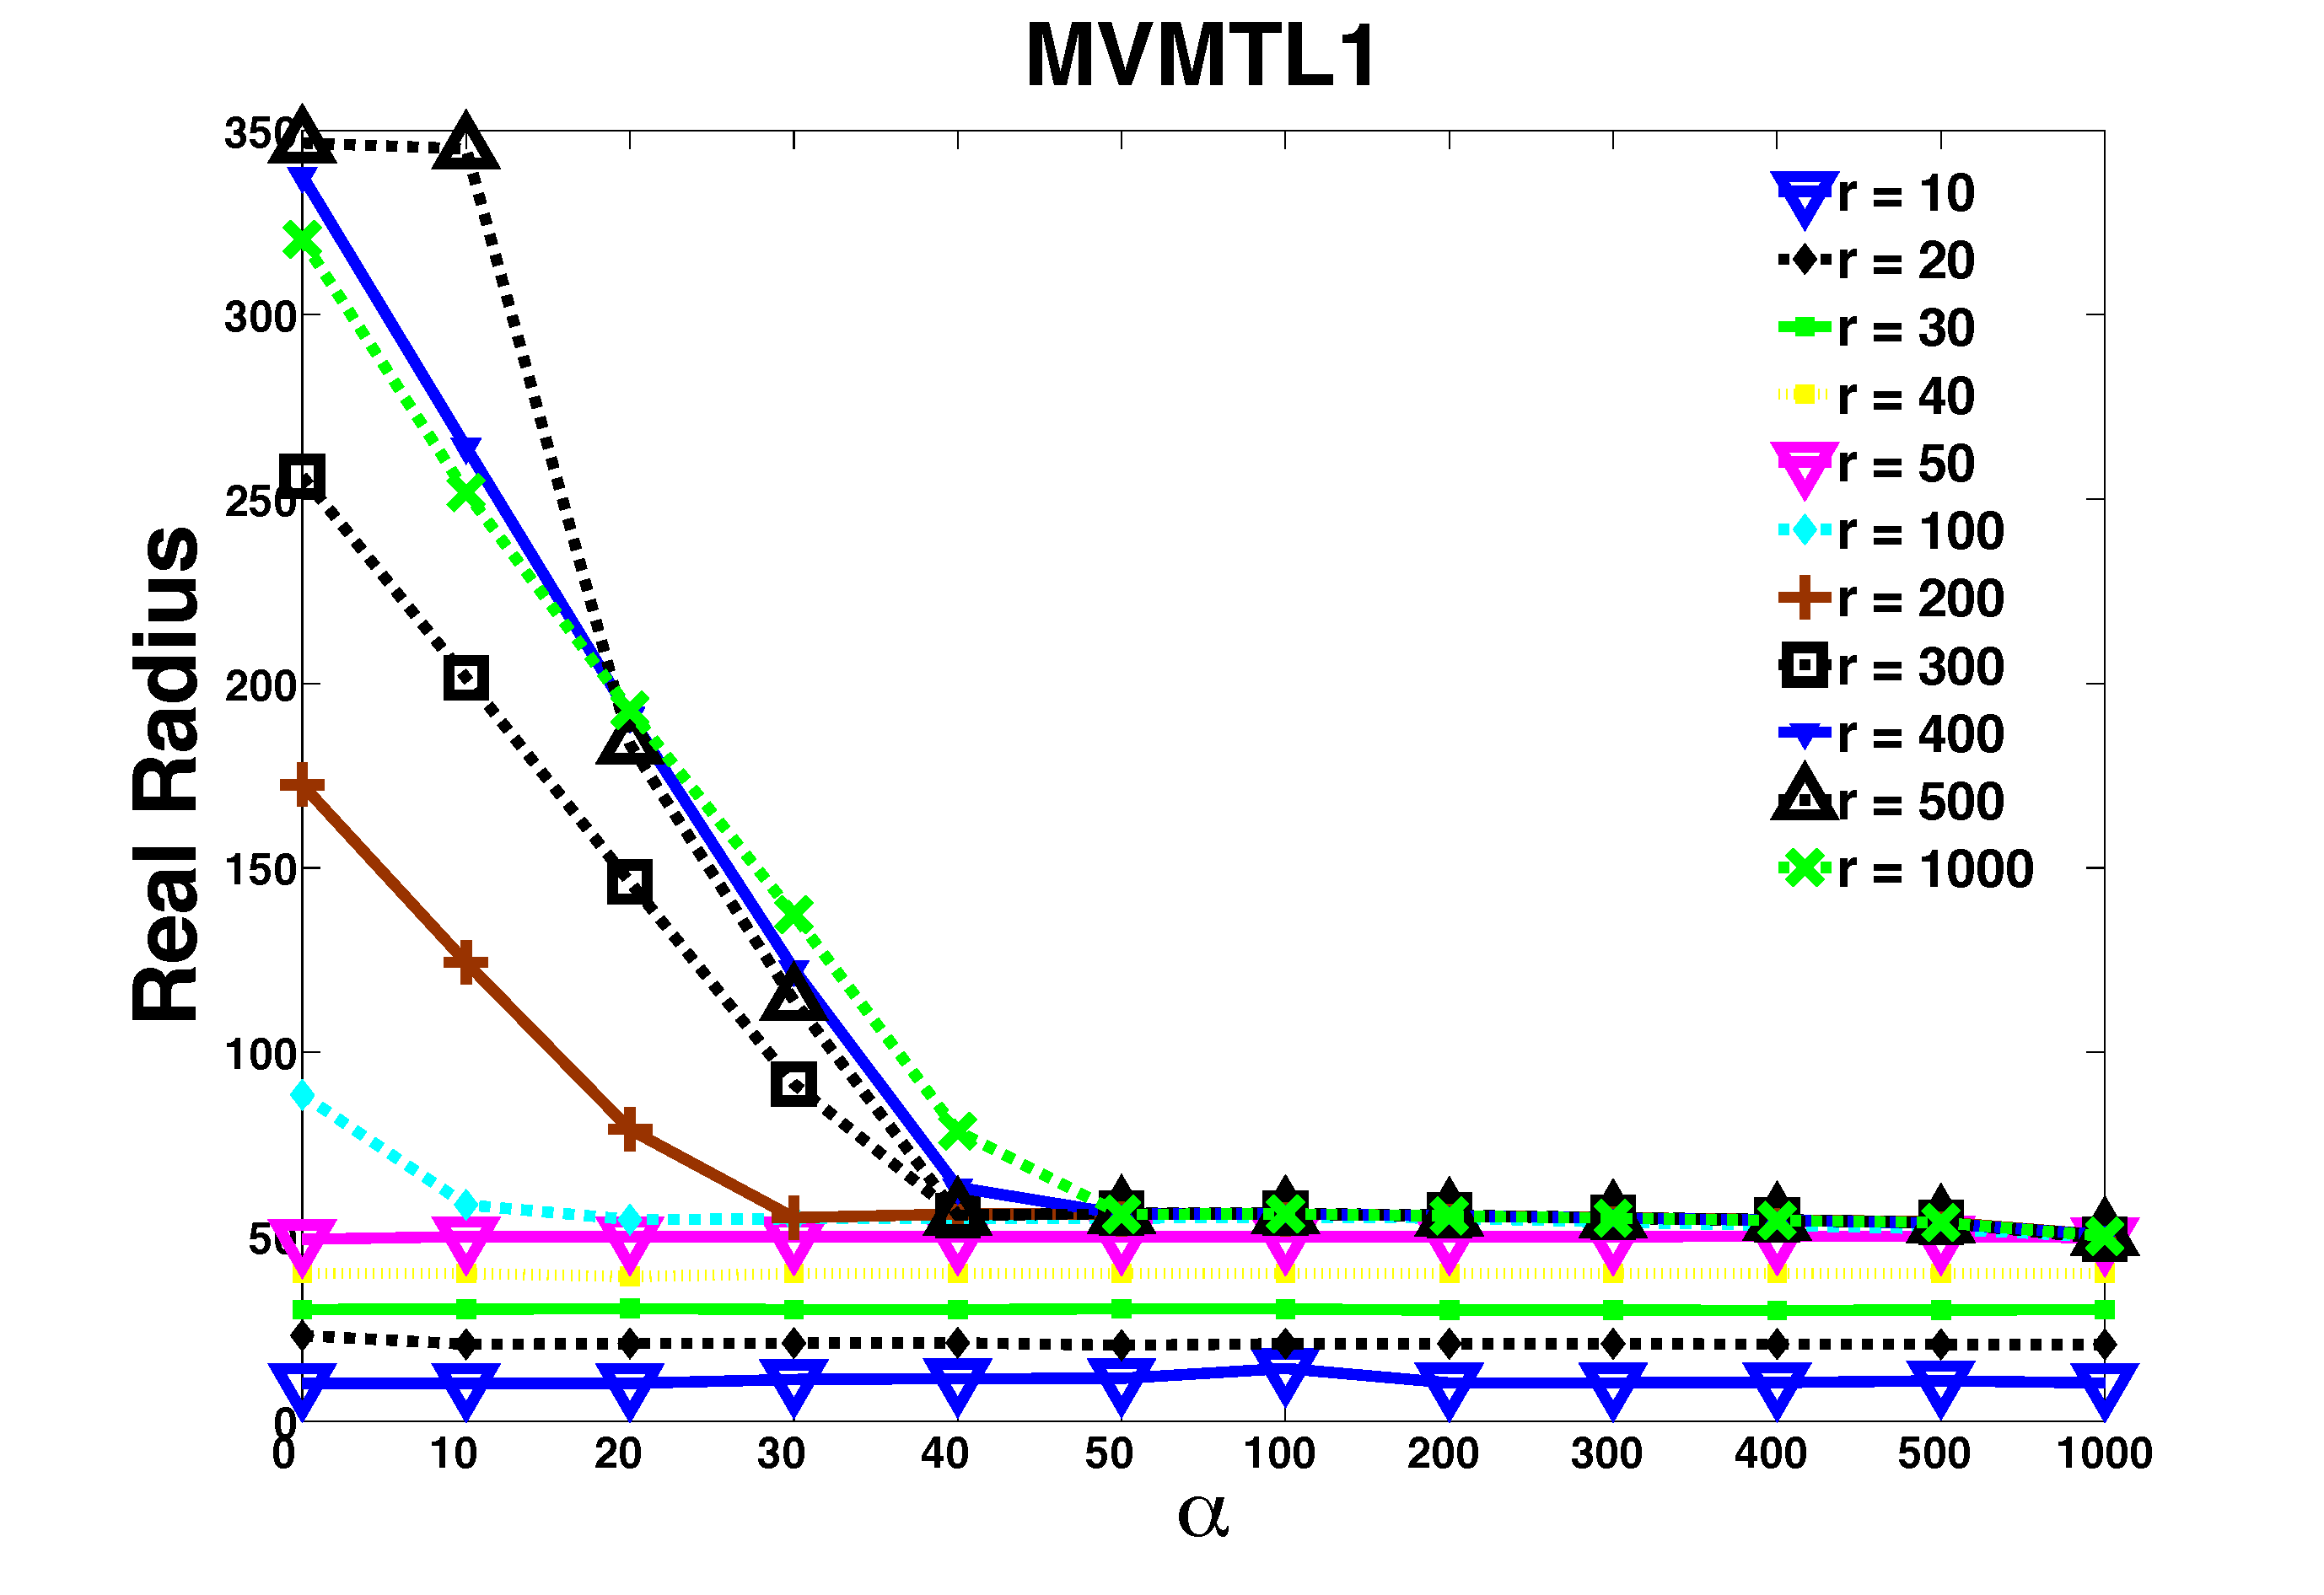
\includegraphics[width= .5\textwidth, height=1.3in]{figures/alpha_mvmtl1.pdf}\\
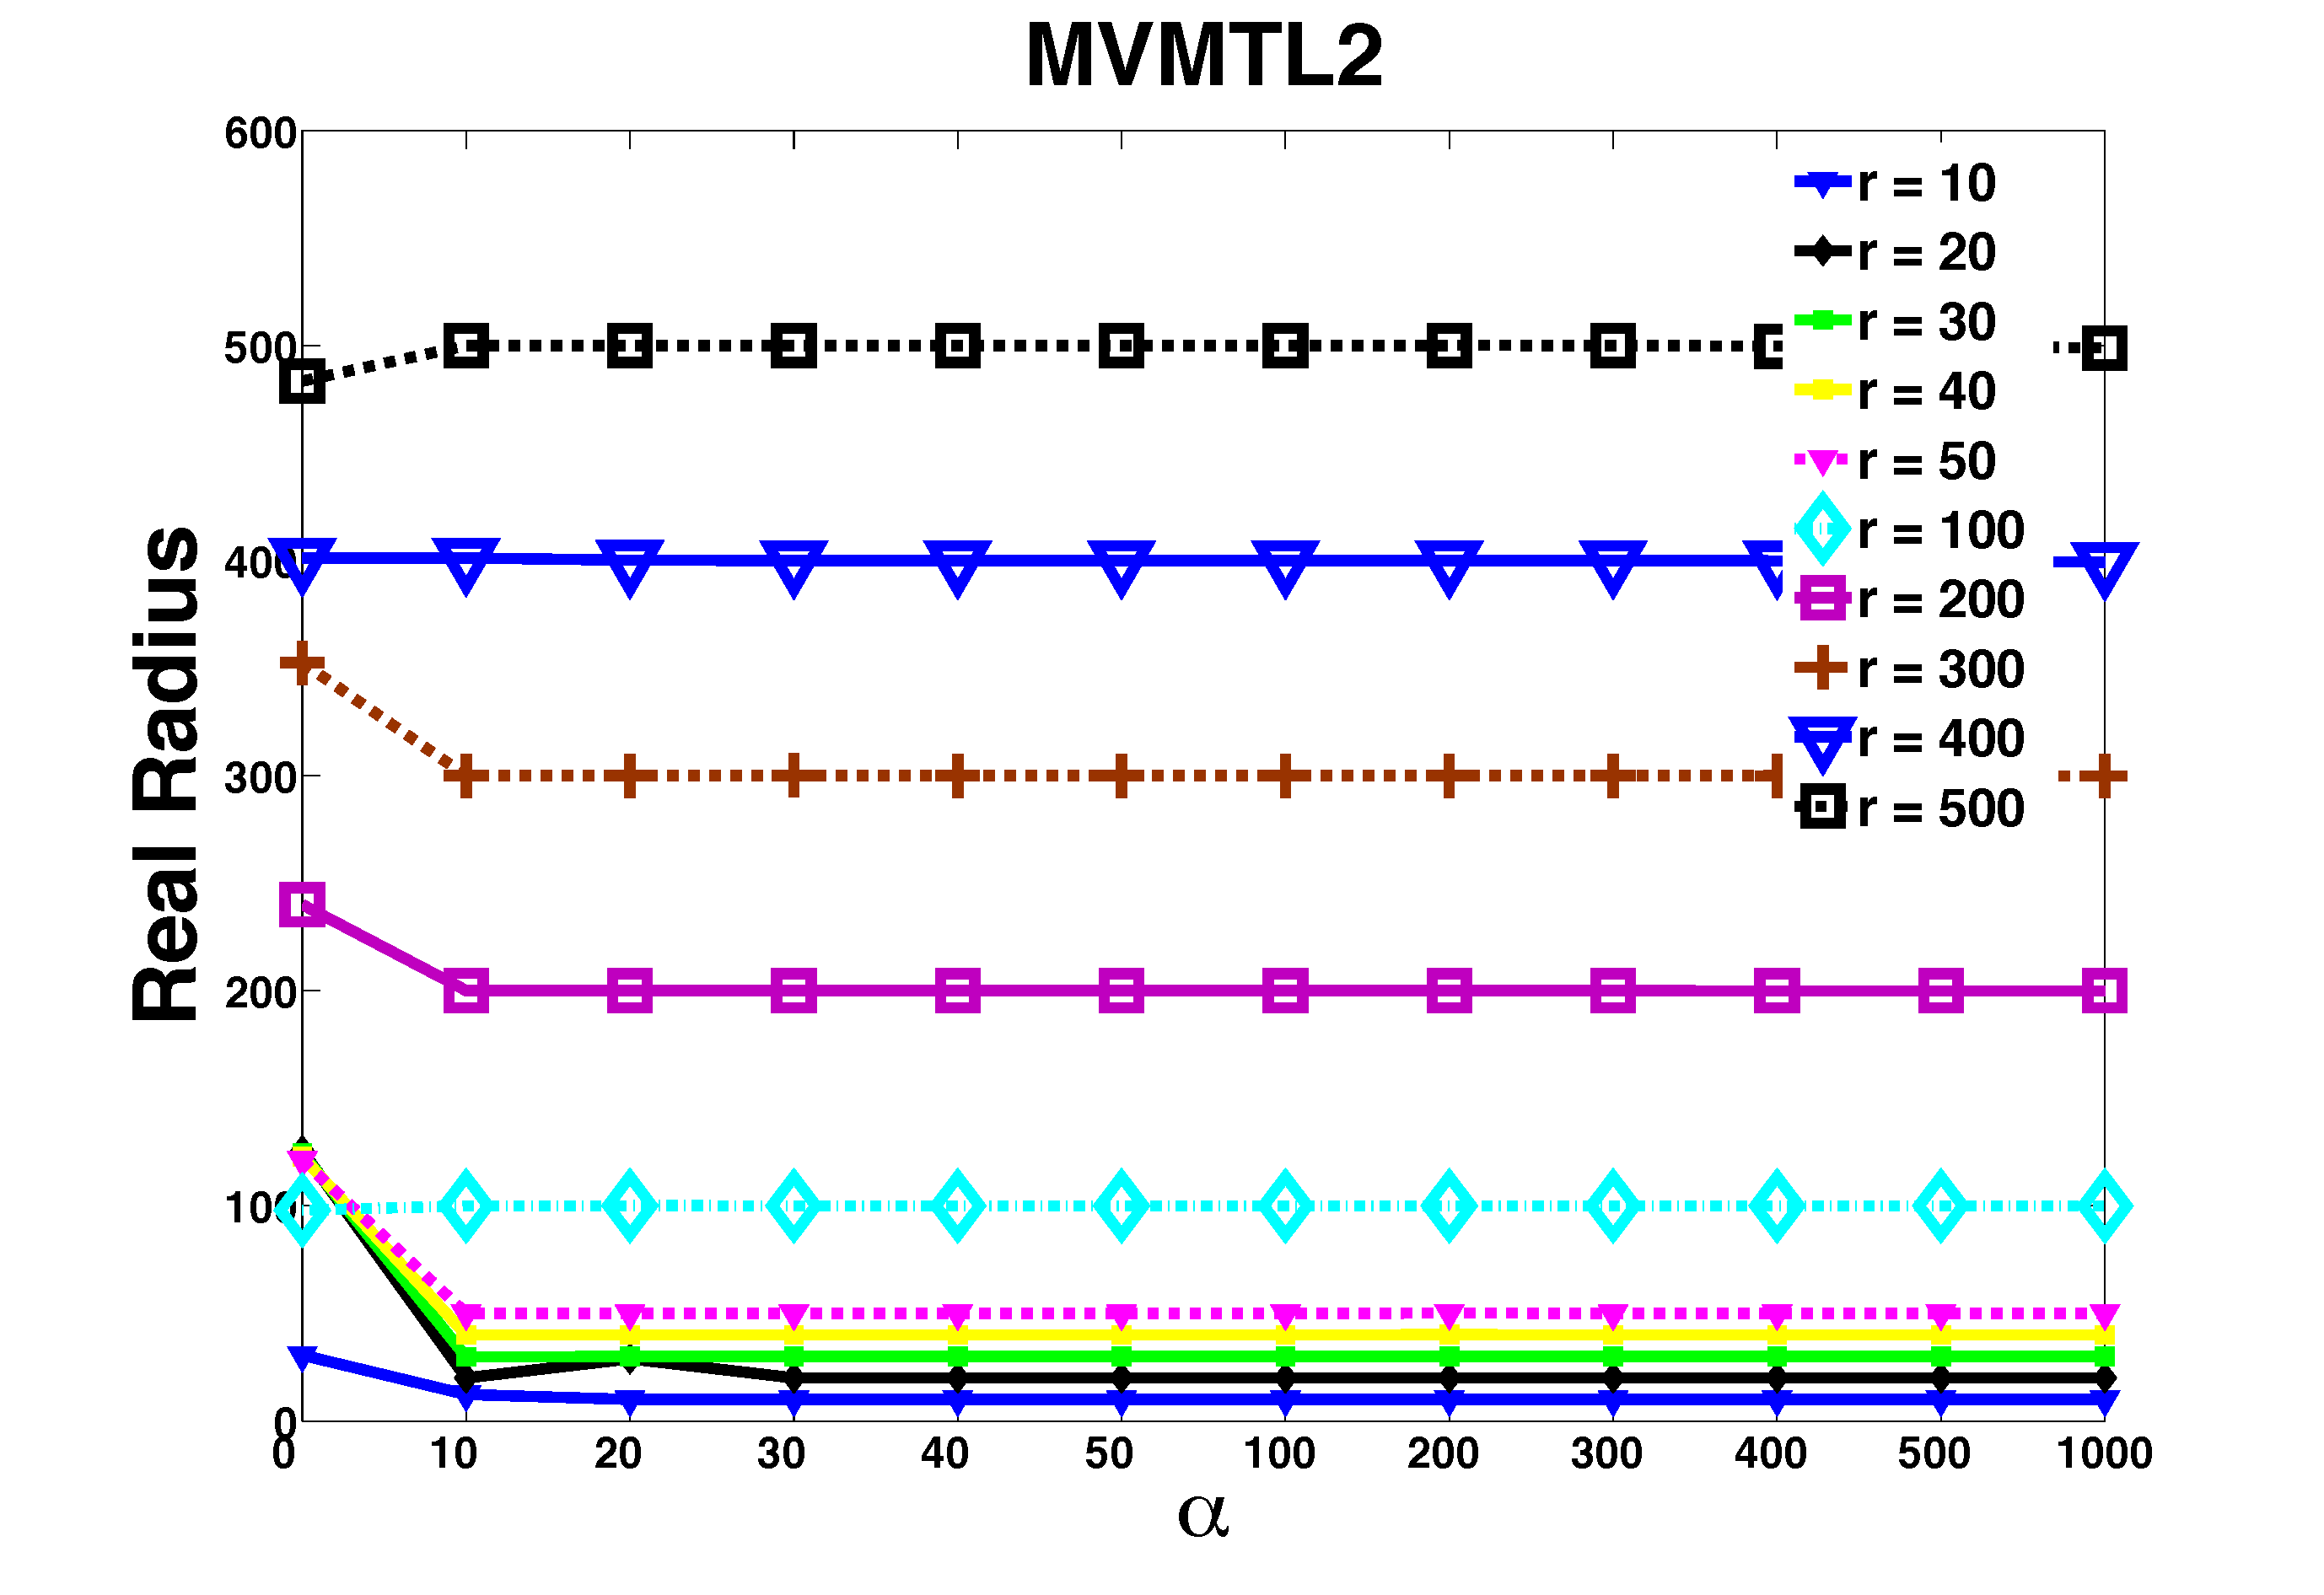
\includegraphics[width= .5\textwidth, height=1.3in]{figures/alpha_mvmtl2.pdf}
\end{minipage}
\caption{Radius Control Comparison w.r.t $\alpha$}
\label{fig:v-alpha}
\end{figure}
%%
\begin{figure}
\begin{center}
\begin{minipage}{1\textwidth}
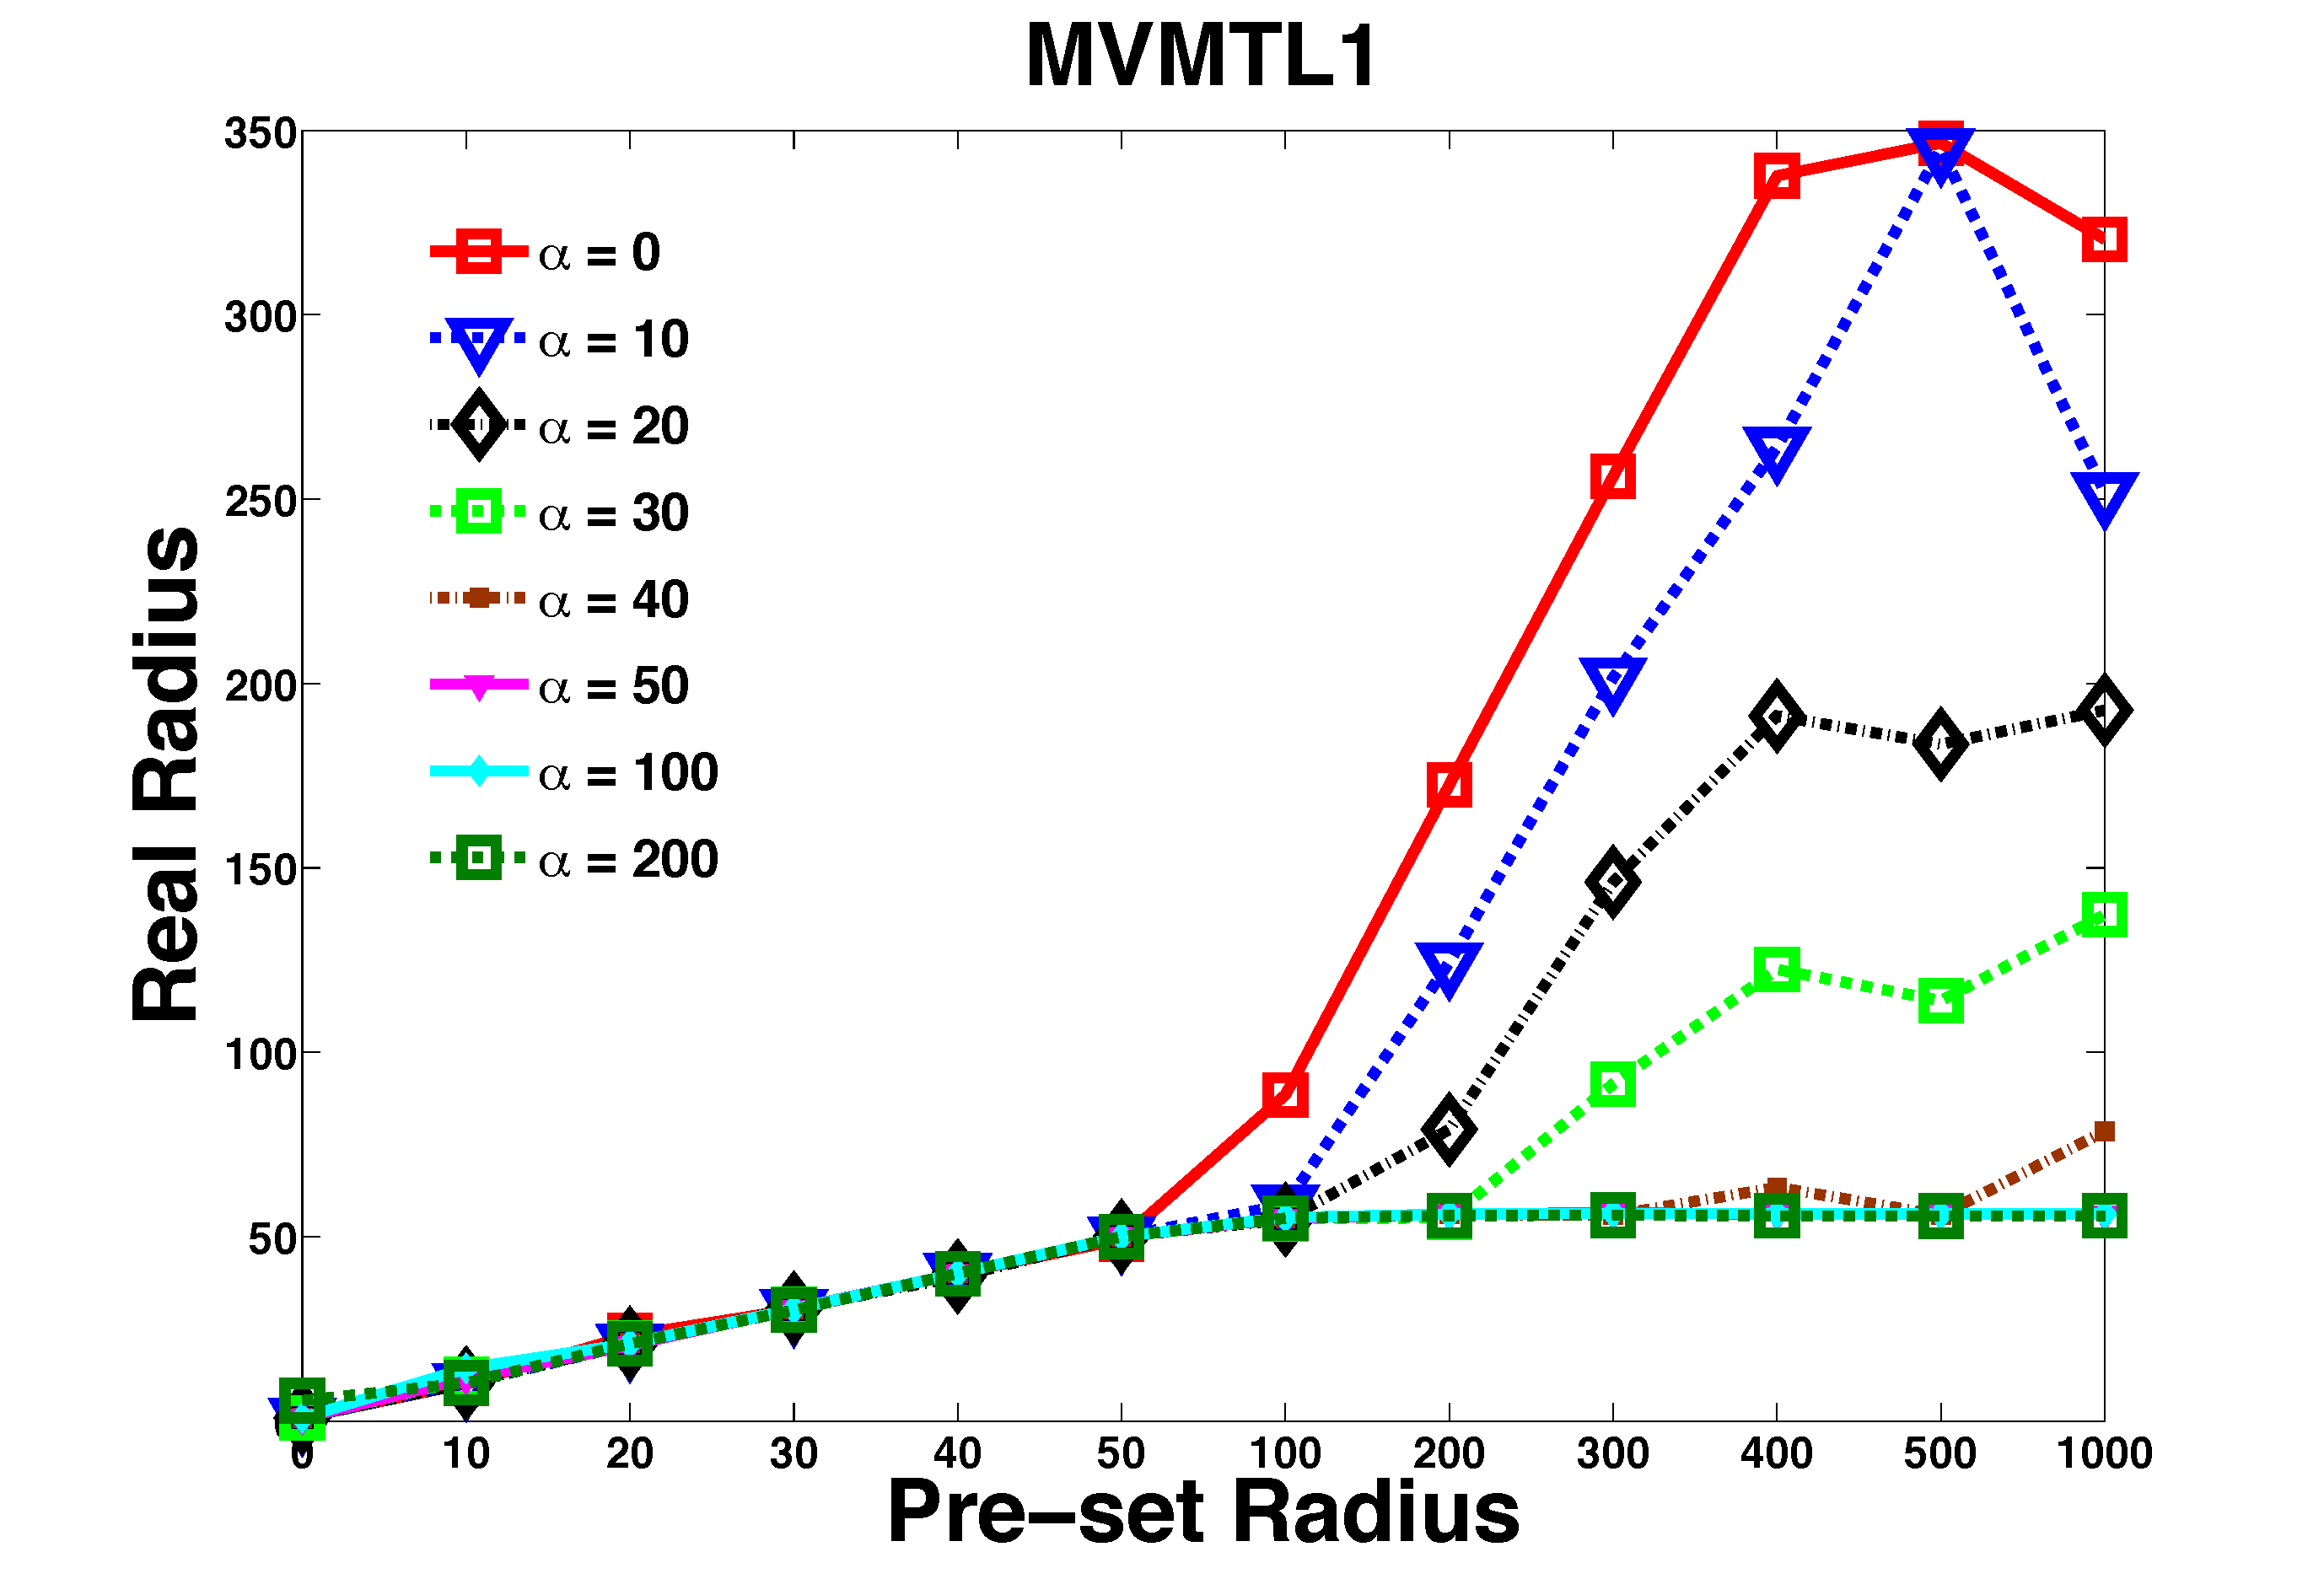
\includegraphics[width= .25\textwidth, height=1.6in]{figures/radius_mvmtl1.pdf}
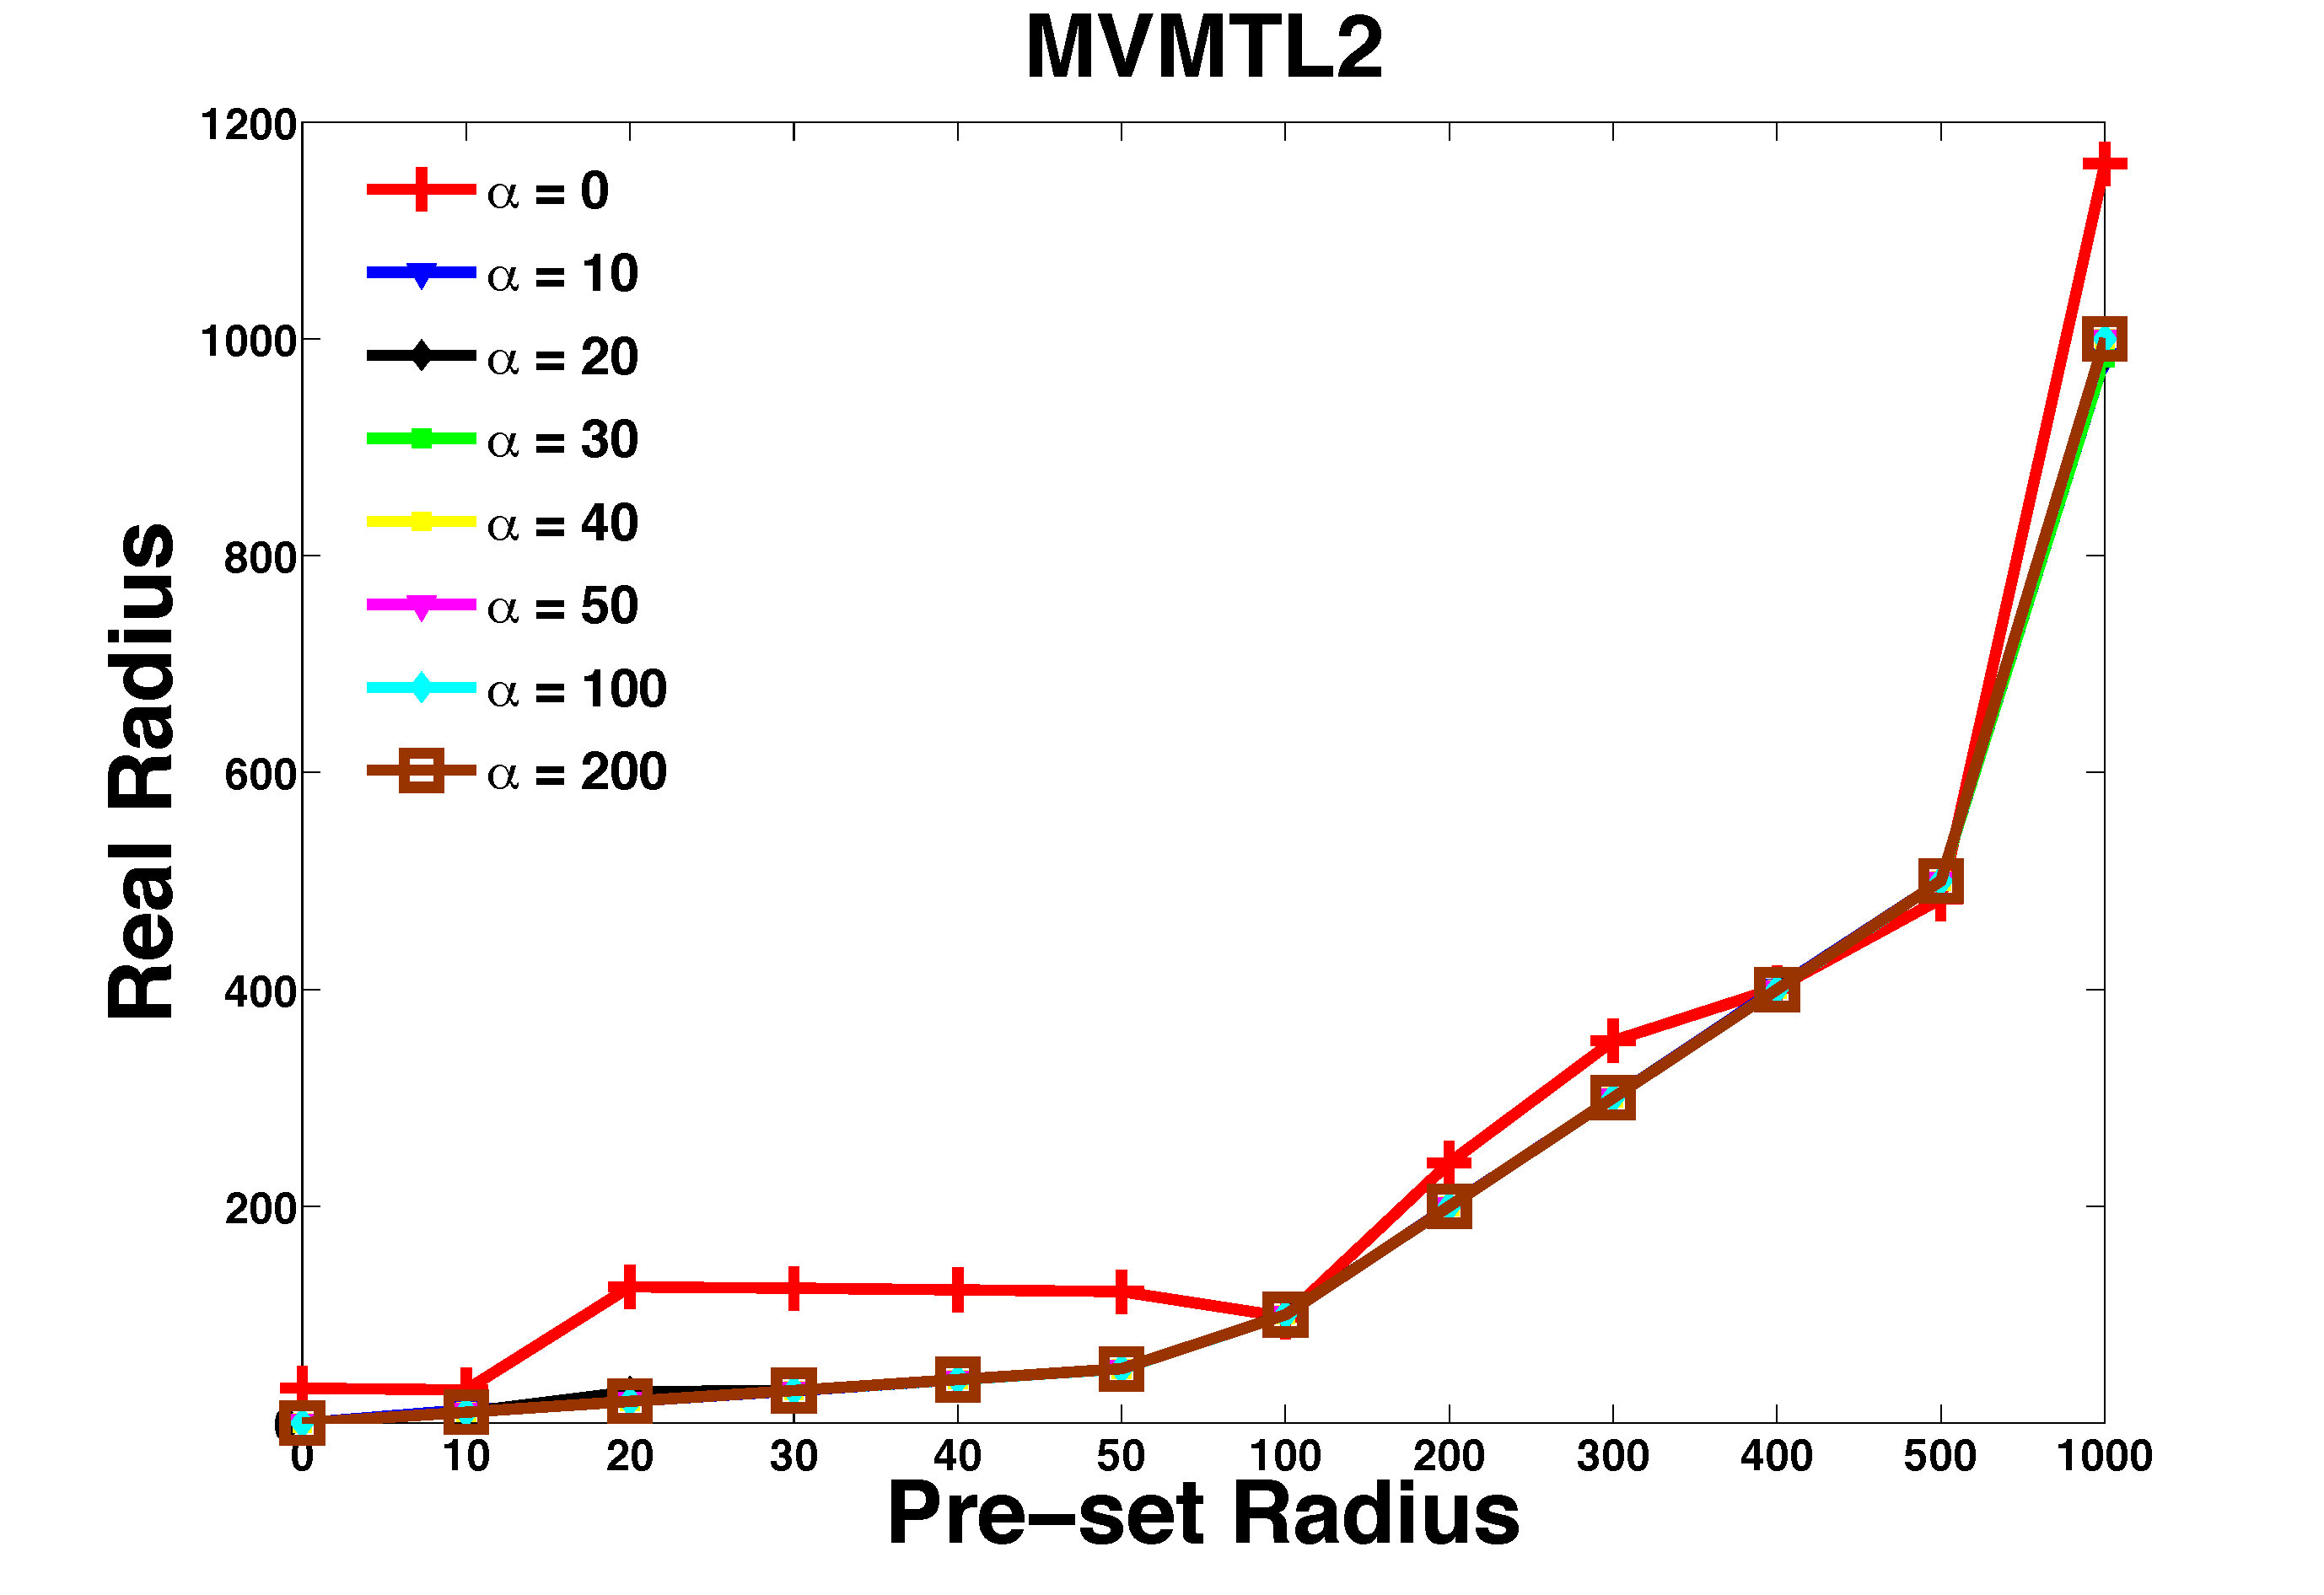
\includegraphics[width= .25\textwidth, height=1.6in]{figures/radius_mvmtl2.pdf}
\end{minipage}
\end{center}
\caption{Radius Control Comparison w.r.t Different Pre-set Radiuses}
\label{fig:v-radius}
\end{figure}
%

\subsection{Sensitivity Studies on Parameters }
%
This experiment conducts the sensitivity study of the proposed
algorithm to the parameter $\alpha$. The result of MVMTL1 is shown in Figure \ref{fig:sensitivity}.
For each $\alpha$, cross-validation is utilized to find out the best $r$. We randomly split the School data into $10\% :90\% $, where $10\%$ is used for training, and the rest $90\%$ is used for testing. The result is shown in Figure \ref{fig:sensitivity}, where the elbow effect is shown in choosing parameter $\alpha$. The result for MVMTL2 is similar and is thus not shown due to space limitations.
%
\begin{figure}[htb]
\begin{minipage}{1\textwidth}
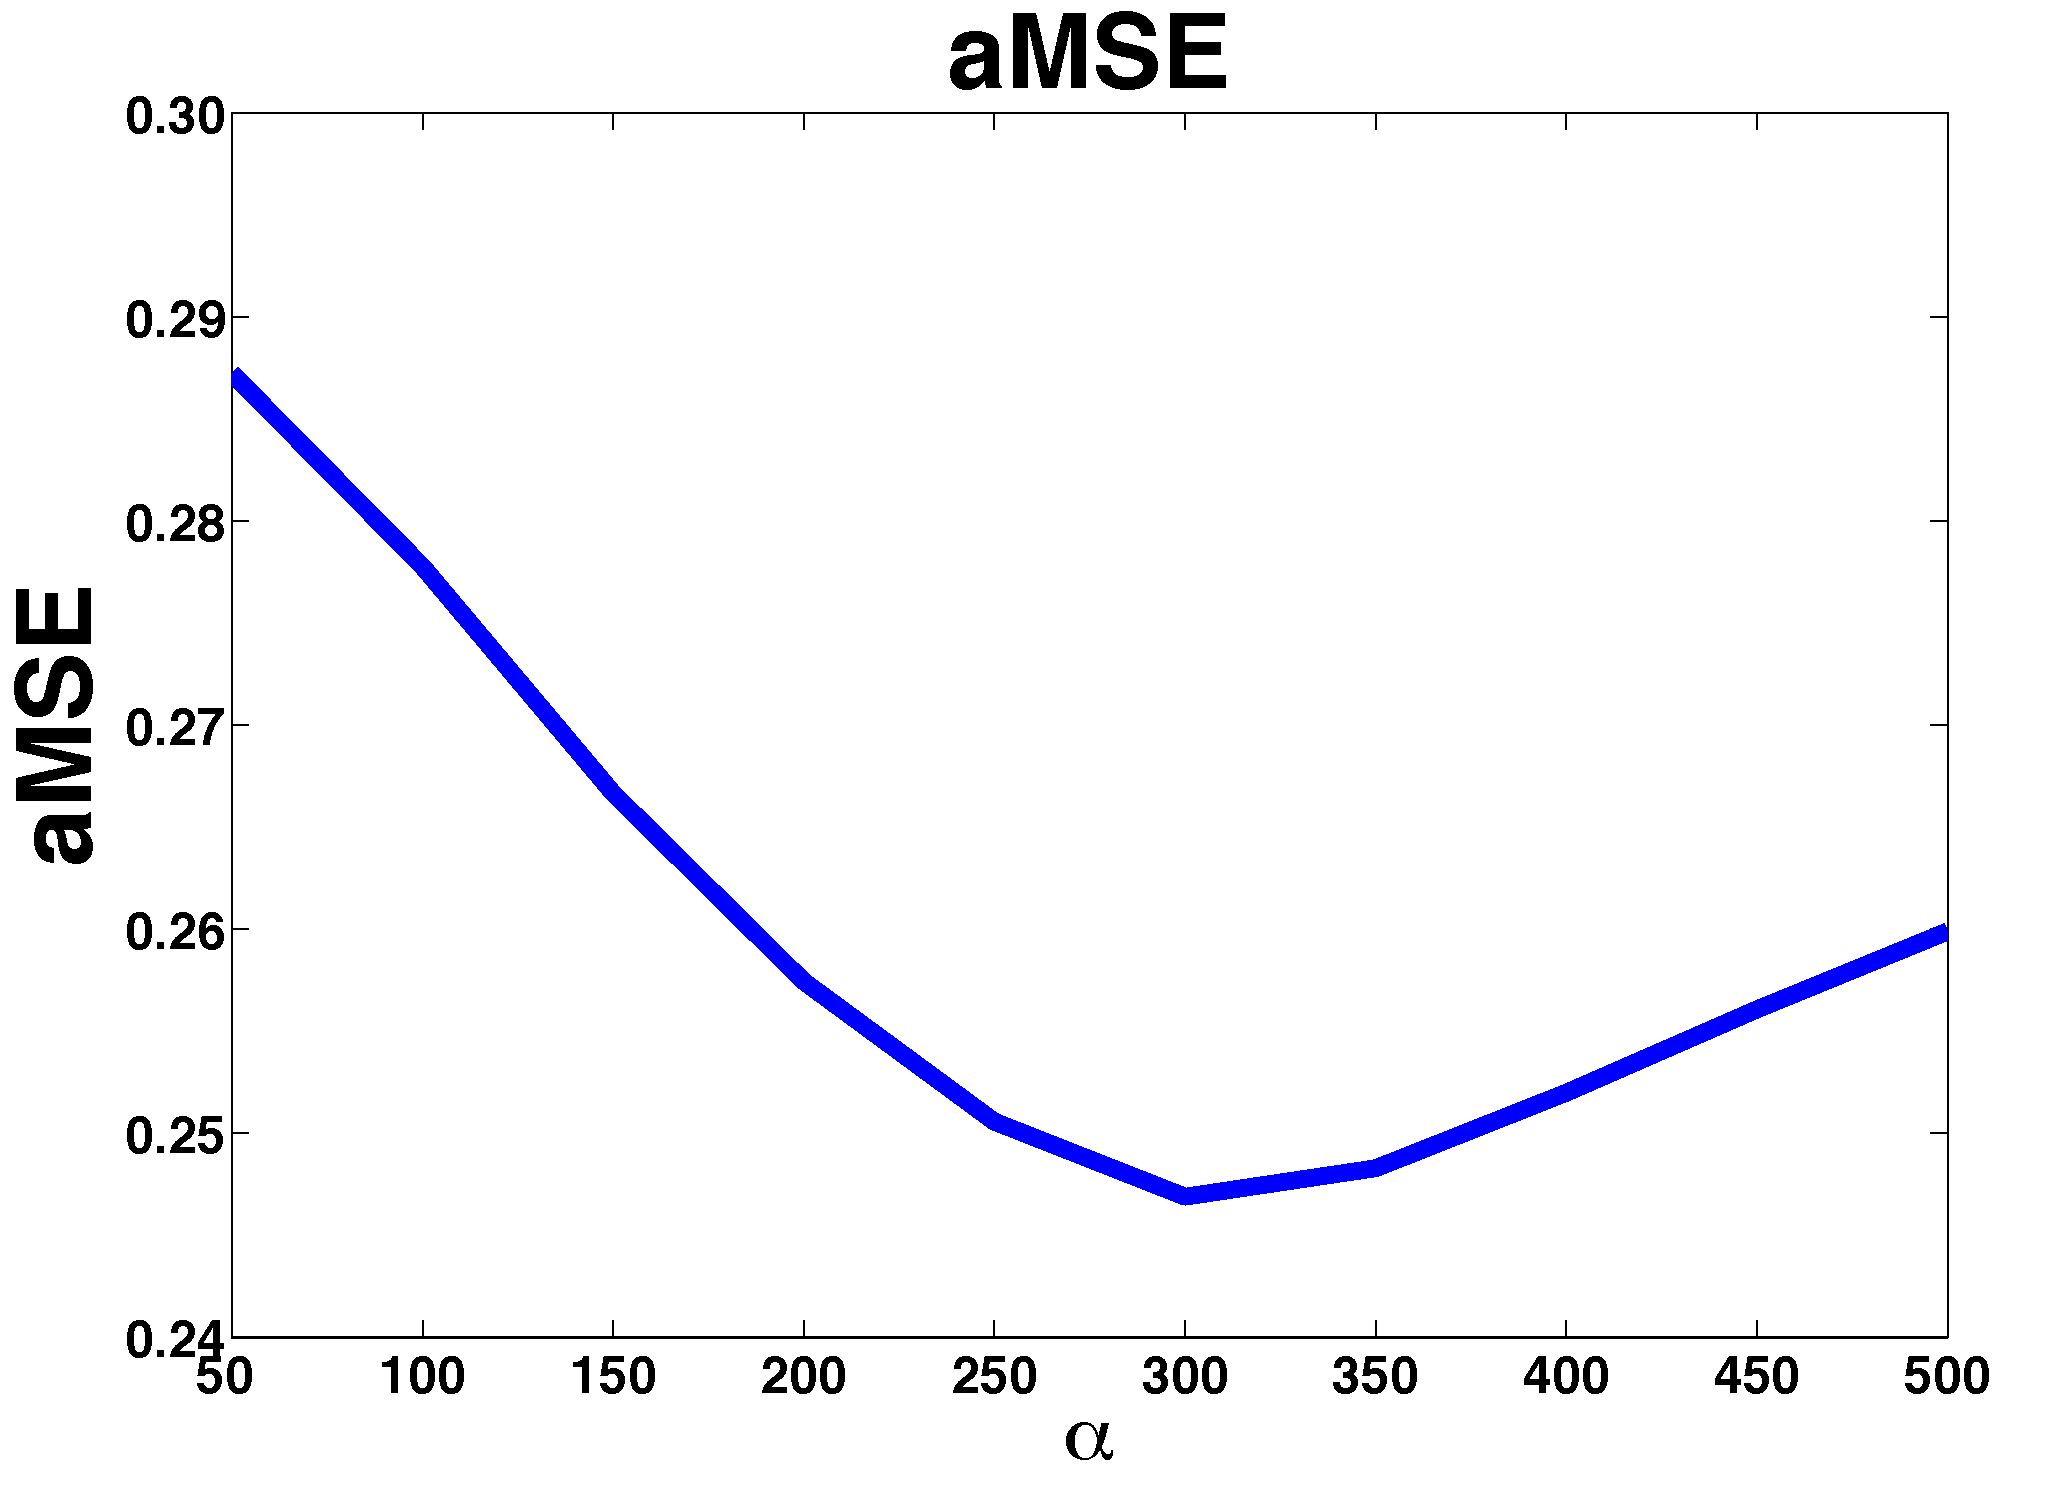
\includegraphics[width= .24\textwidth, height=.8in]{figures/AMSE.pdf}
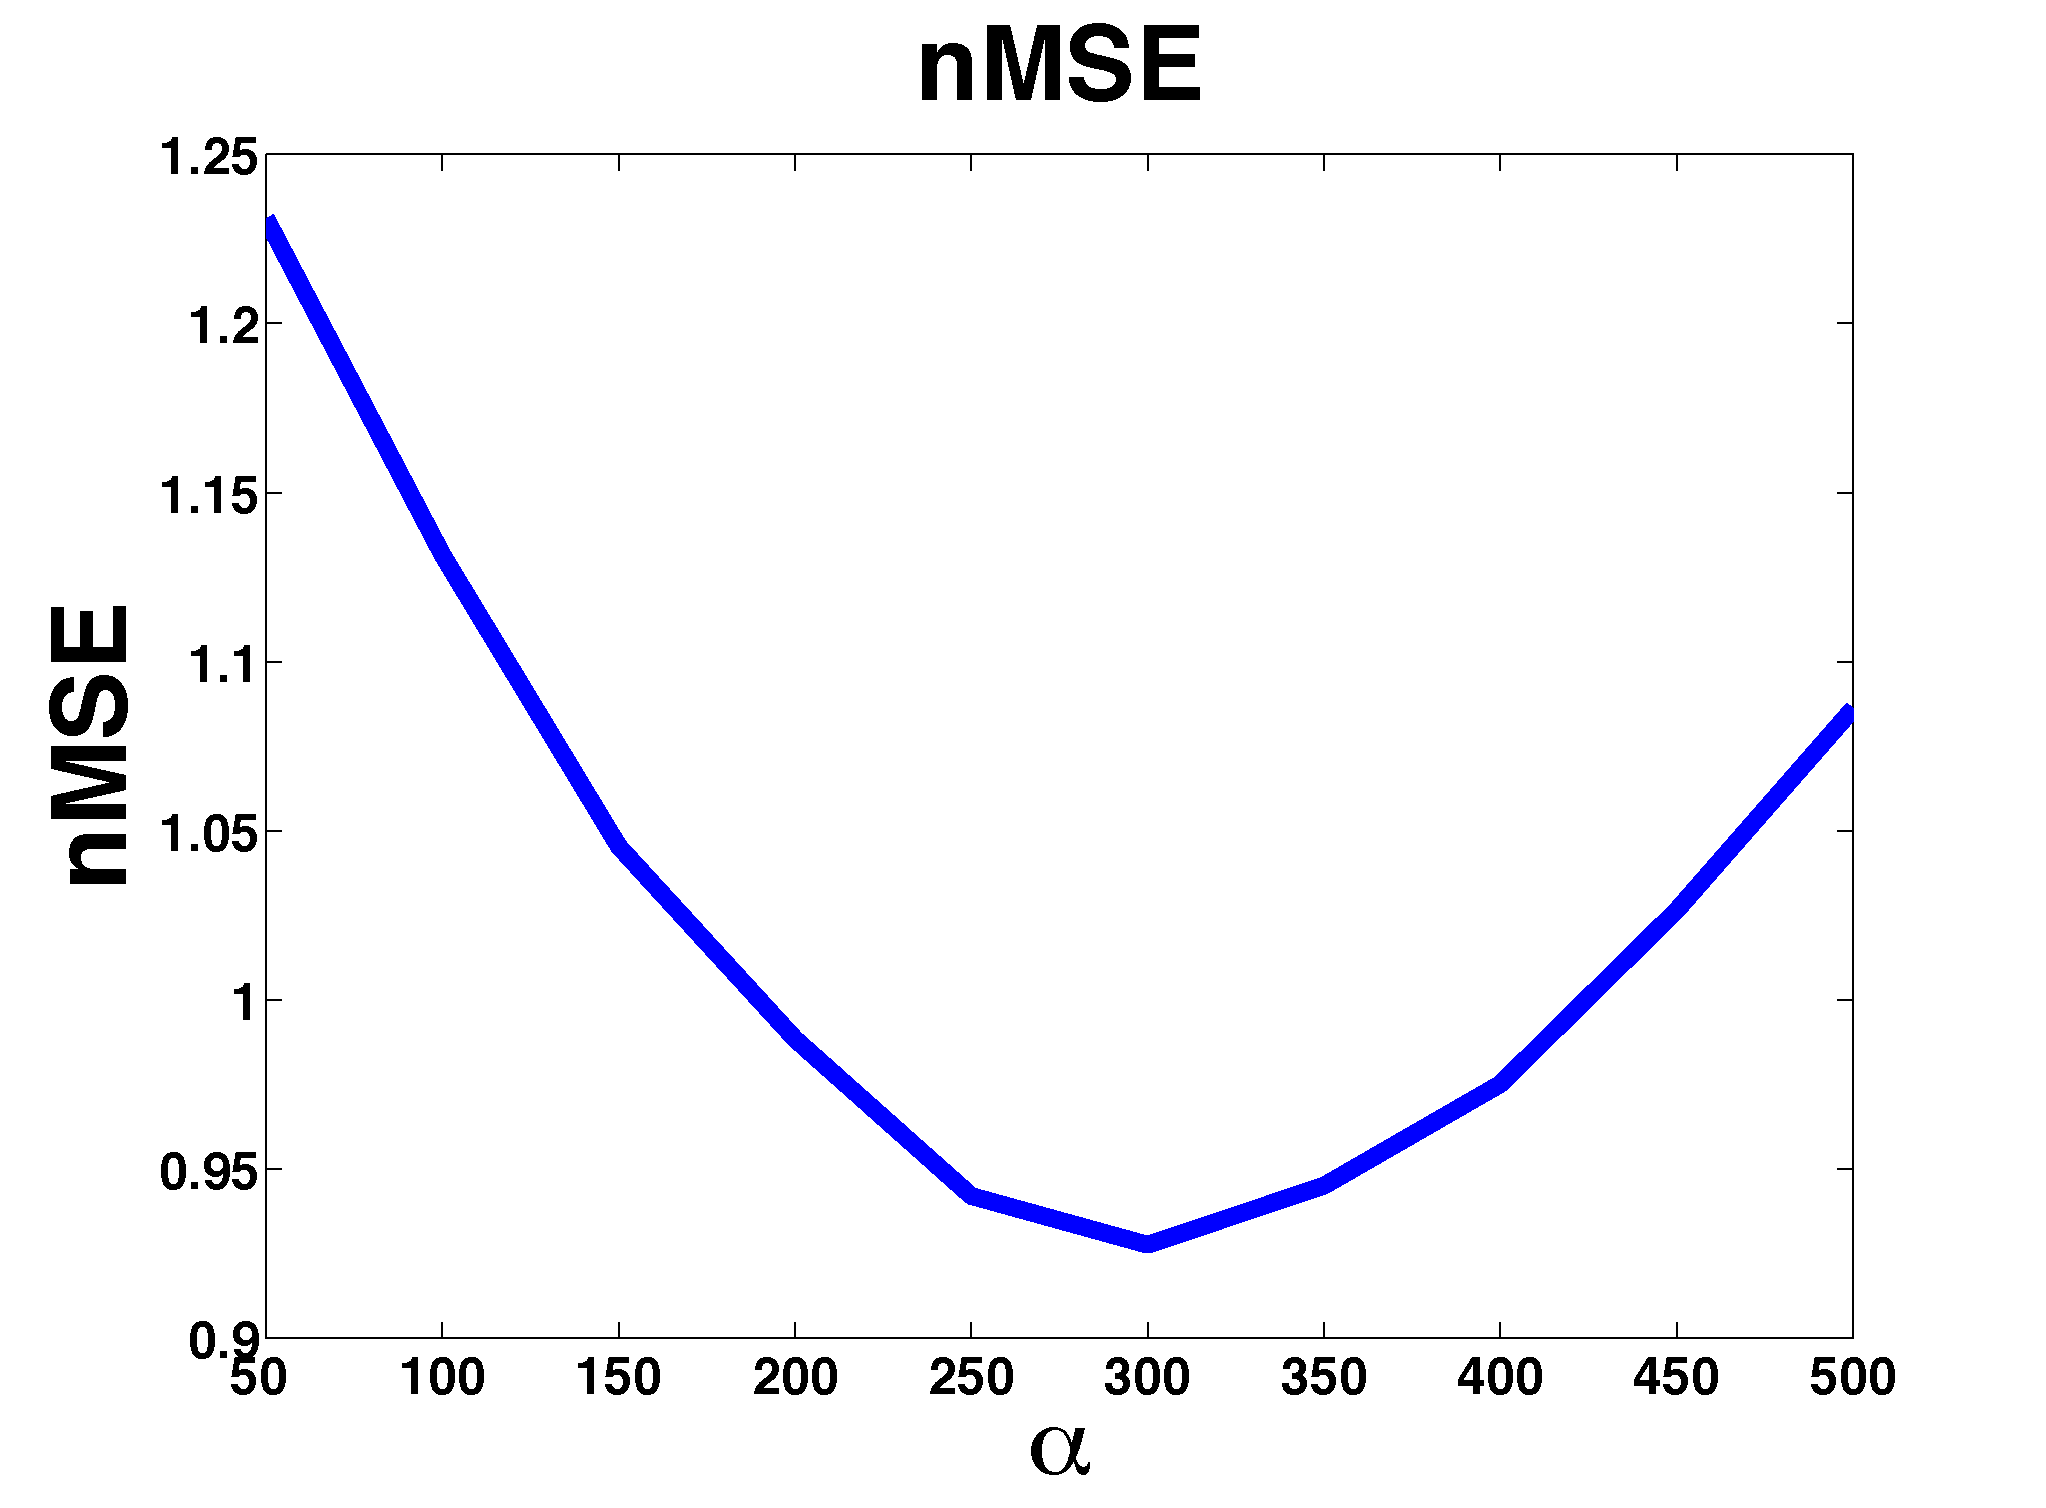
\includegraphics[width= .24\textwidth, height=.8in]{figures/NMSE.pdf}\\
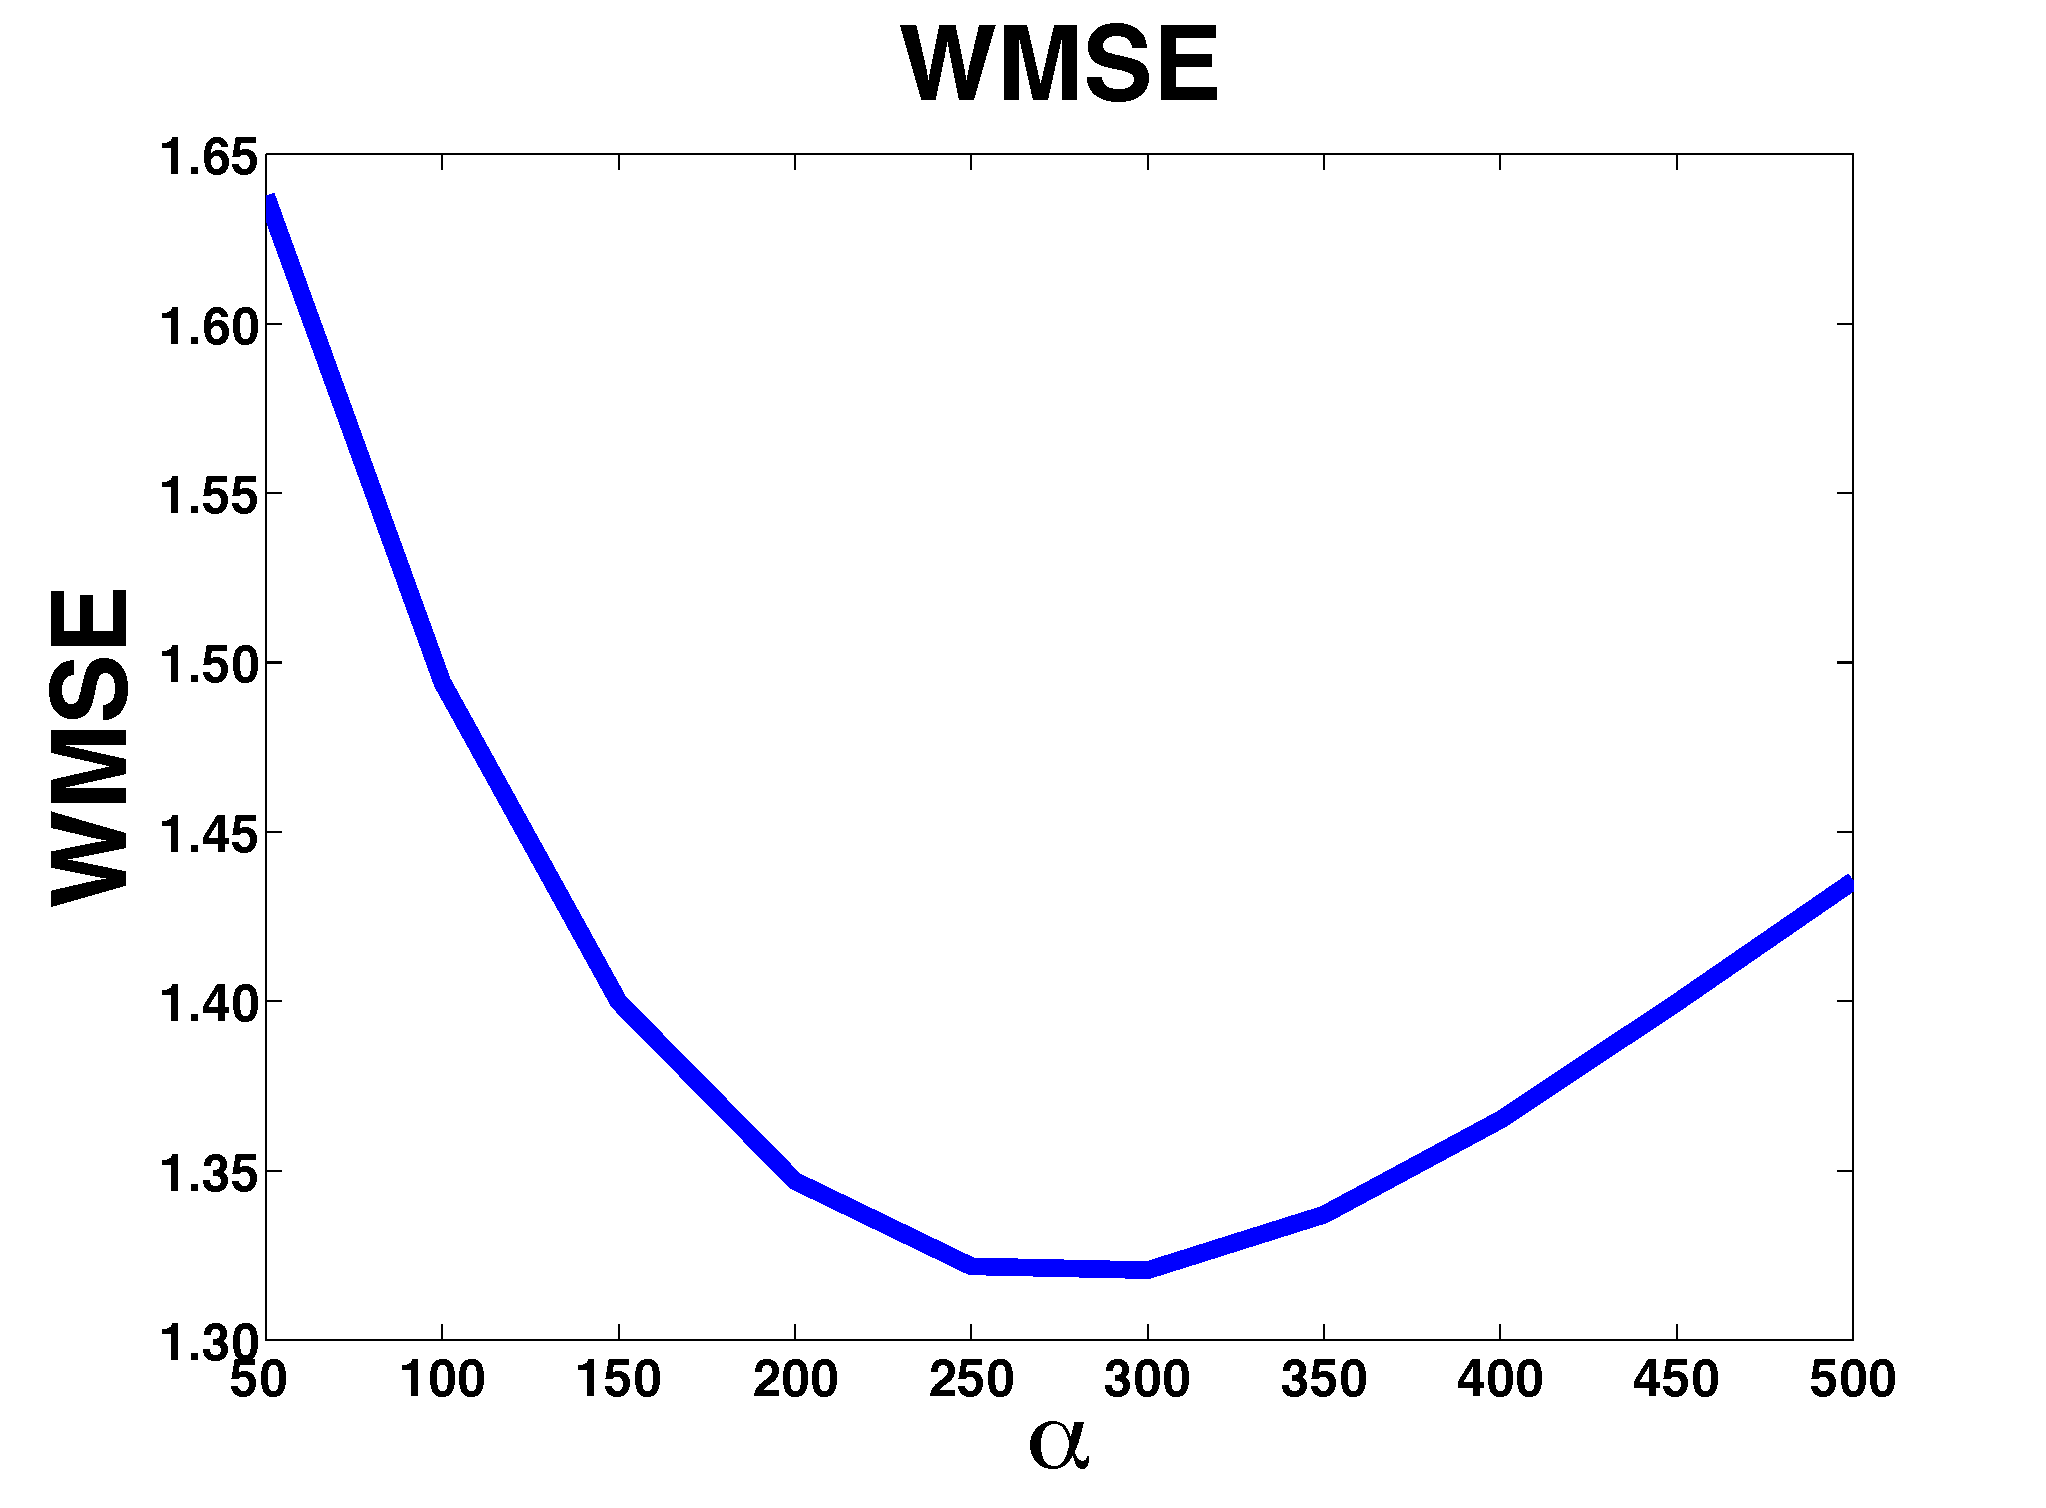
\includegraphics[width= .24\textwidth, height=.8in]{figures/WMSE.pdf}
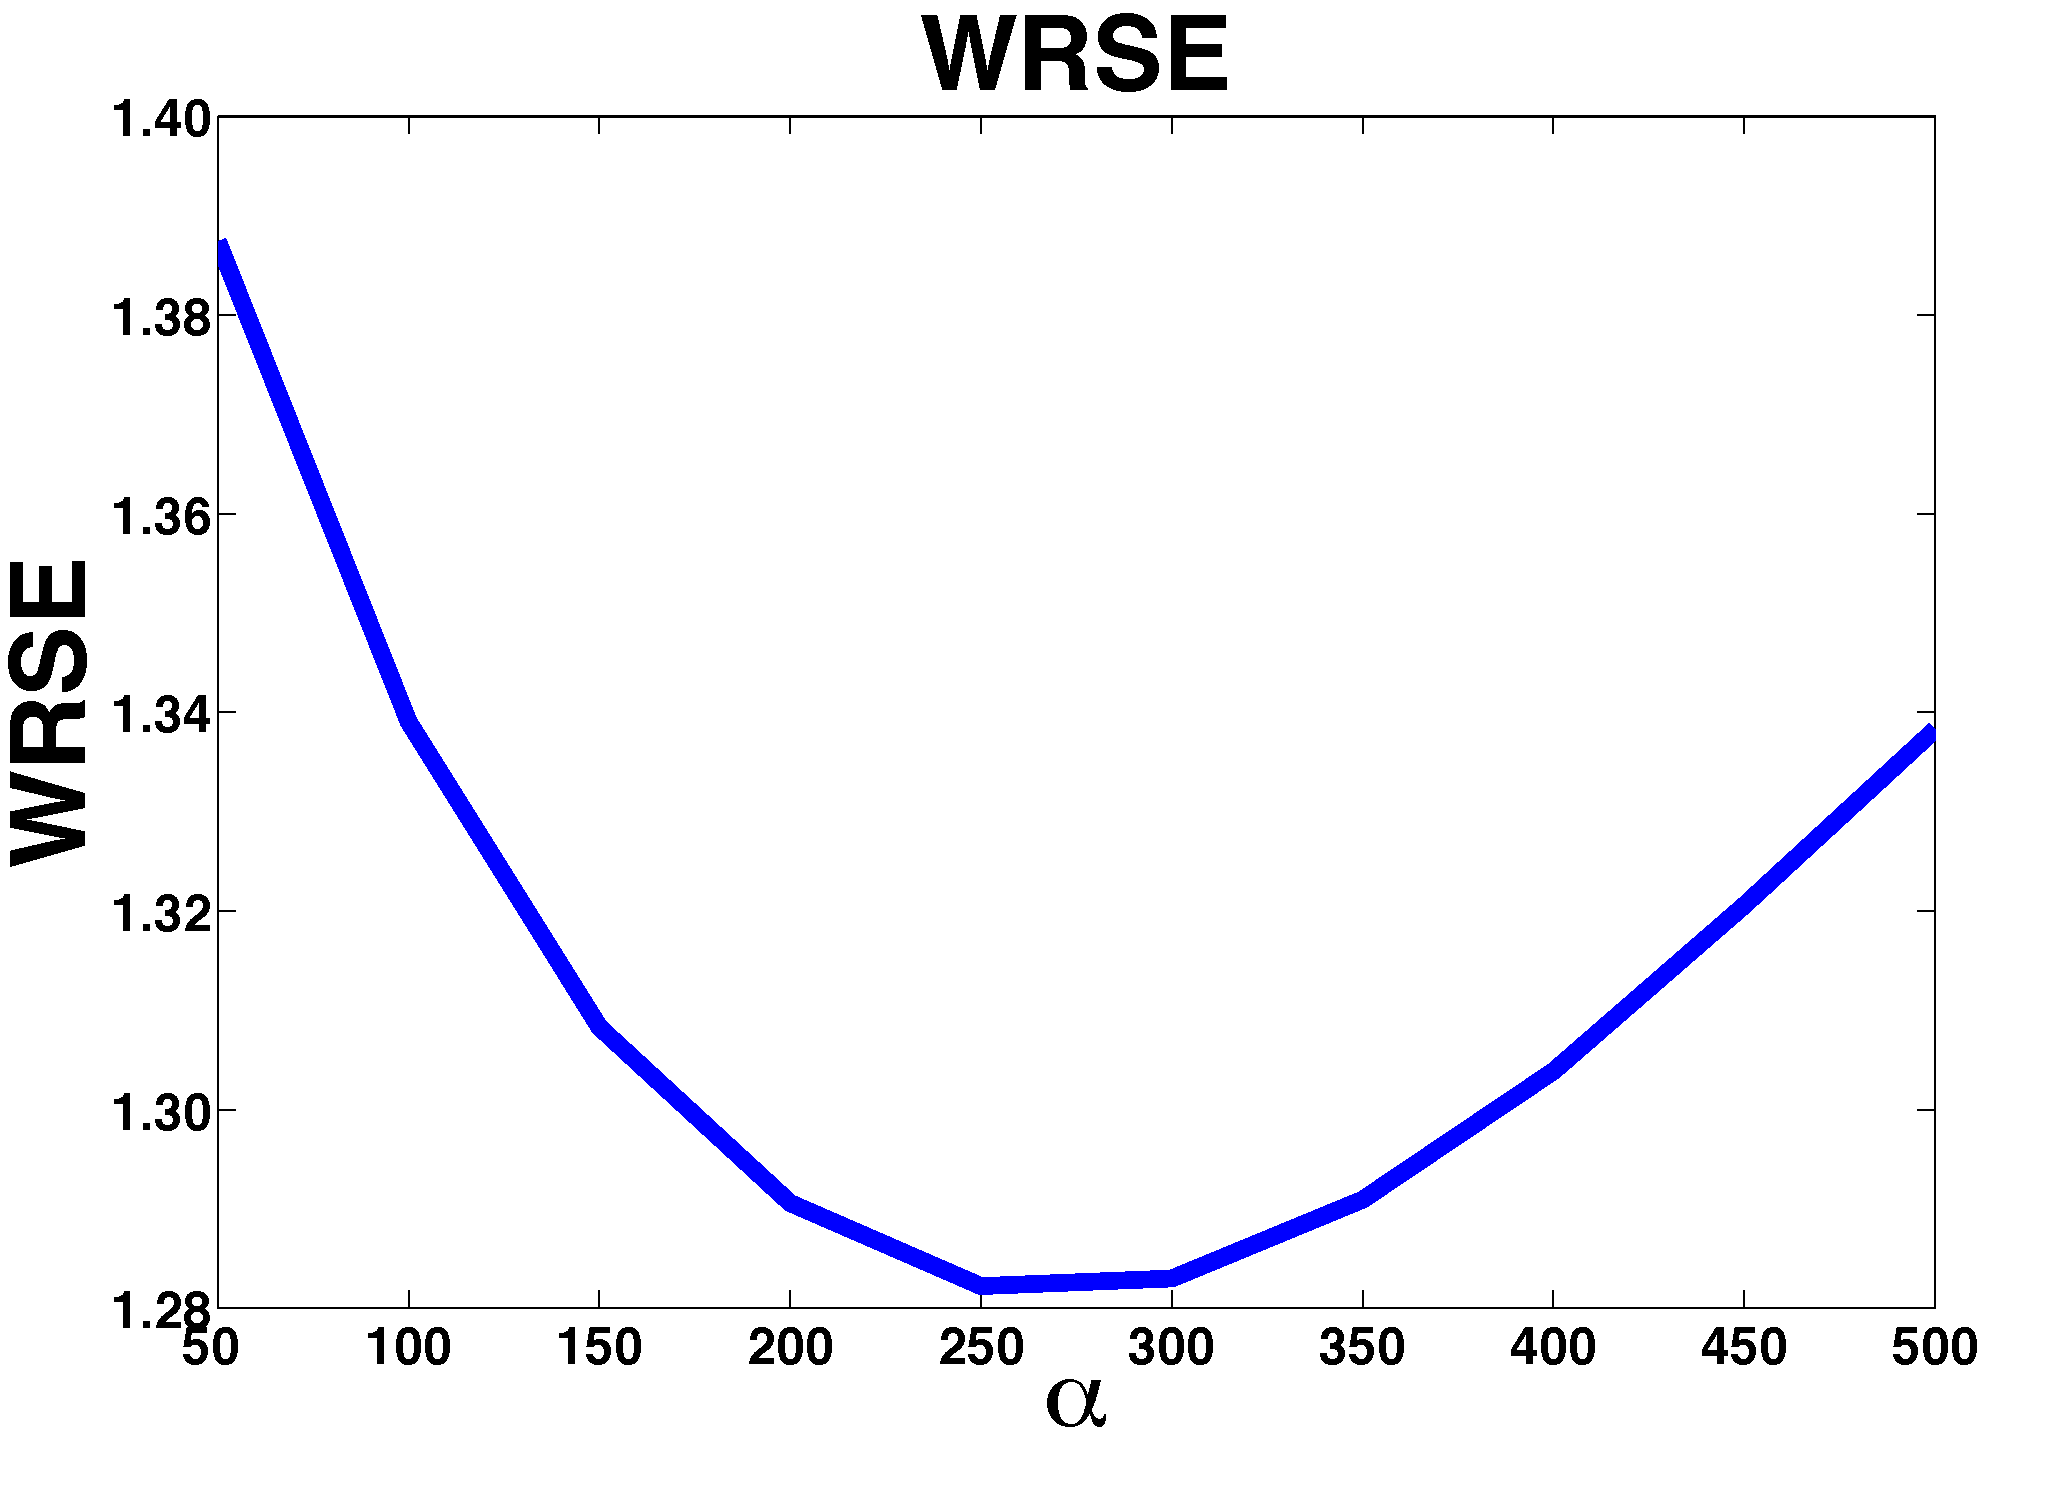
\includegraphics[width= .24\textwidth, height=.8in]{figures/WRSE.pdf}
\end{minipage}
\caption{Sensitivity Performance w.r.t $\alpha$}
\label{fig:sensitivity}
\end{figure}
%
%
%\begin{table*}[h]
%\begin{tabular}{|c|c|c|c|c|c|c|c|c|}
%\hline 
%method & \multicolumn{4}{c|}{MVMTL1} & \multicolumn{4}{c|}{MVMTL2}\tabularnewline
%\hline 
%\hline 
%sample ratio& aMSE & nMSE & WMSE & WRSE & aMSE & nMSE & WMSE & WRSE\tabularnewline
%\hline 
%10\% & 0.2481 & 0.9216 & 1.3210 & 1.2835 & 0.2364  & 0.8784 & 1.3383 & 1.2177\tabularnewline
%\hline 
%20\% & 0.2185 & 0.8156 & 1.2057 & 1.2184 & 0.2047 & 0.8056 & 1.2437 & 1.1824\tabularnewline
%\hline 
%30\% & 0.1951 & 0.7669 & 1.1551 & 1.1640 & 0.1844  & 0.7542 & 1.1179 & 1.0608\tabularnewline
%\hline 
%40\% & 0.1874 & 0.7534 & 1.1858 & 1.0843 & 0.1765 & 0.7364 & 1.0422 & 0.9624\tabularnewline
%\hline 
%50\% & 0.1802 & 0.7349 & 1.0947 & 0.9951 & 0.1683 & 0.7240 & 0.9093 & 0.8638\tabularnewline
%\hline 
%60\% & 0.1723 & 0.7267 & 0.9824 & 0.9218 & 0.1617 & 0.7165 & 0.8735 & 0.7541\tabularnewline
%\hline 
%70\% & 0.1614 & 0.7126 & 0.9246 & 0.8115 & 0.1559 & 0.6943 & 0.8639 & 0.7102\tabularnewline
%\hline 
%\end{tabular}
%\caption{Sample Complexity Comparison on School Data}
%\label{tab: sample_school}
%\end{table*}
%
\begin{table*}[htb]
\begin{tabular}{|p{1cm}|c|c|c|c|c|c|c|c|c|c|c|c|}
\hline 
\small School& \multicolumn{3}{c|}{aMSE} & \multicolumn{3}{c|}{nMSE} & \multicolumn{3}{c|}{WMSE} & \multicolumn{3}{c|}{WRSE}\tabularnewline
\hline 
\tiny samples & 10\% & 20\% & 30\% & 10\% & 20\% & 30\% & 10\% & 20\% & 30\% & 10\% & 20\% & 30\%\tabularnewline
\hline 
\tiny Trace & 0.2504 & 0.2156 & 0.2089 & 0.9359 & 0.8211 & 0.7870 & \textbf{1.3241} & 1.1773 & 1.1726 & \small \textbf{1.2088} & 1.0859 & 1.0117\tabularnewline
\hline 
\tiny Lasso & 0.2682 & 0.2289 & 0.2137 & 1.0261 & 0.8754 & 0.8144 & 1.4940 & 1.3079 & 1.2769 & 1.2759 & 1.1338 & 1.0543\tabularnewline
\hline 
\tiny RMTL & 0.2330 & \small\textbf{0.2018} & 0.1844 & 0.9130 &\small\textbf{ 0.8055} & 0.7600 & 1.3267 & 1.1767 & 1.1201 & 1.2131 & \small\textbf{1.0844} & 1.0127\tabularnewline
\hline 
\tiny L21 & 0.2735  & 0.2218 & 0.1903  & 1.0173 & 0.8549 & 0.8206 & 1.3986 & 1.2249 & 1.2206 & 1.2968 & 1.1089 & 1.0364\tabularnewline
\hline 
\tiny MVMTL1 & 0.2510  & 0.2185 & 0.1951  & 0.9216 & 0.8156 & 0.7669 & 1.3360 & \textbf{1.2057} & 1.1551 & 1.2985 & 1.2184 & 1.0240\tabularnewline
\hline 
\tiny MVMTL2 & \small\textbf{0.2324}  & 0.2047 & \small\textbf{0.1827}  & \small\textbf{0.8784} & 0.8056 & \small\textbf{0.7542} & 1.3383 & 1.2437 & \small\textbf{1.1179} & 1.2177 & 1.1824 & \small\textbf{1.0108}\tabularnewline
\hline 
\end{tabular}
\caption{Performance Comparison on School Data}
\label{tab:per_school}
\end{table*}
%
%
\begin{table*}[htb]
\begin{tabular}{|p{1cm}|c|c|c|c|c|c|c|c|c|c|c|c|c|}
\hline 
\tiny SARCOS & \multicolumn{3}{c|}{aMSE} & \multicolumn{3}{c|}{nMSE} & \multicolumn{3}{c|}{WMSE} & \multicolumn{3}{c|}{WRSE}\tabularnewline
\hline 
\tiny samples & 50 & 100 & 150 & 50 & 100 & 150 & 50 & 100 & 150 & 50 & 100 & 150\tabularnewline
\hline 
\tiny Trace & 0.1122 & 0.0805 & 0.0772 & 0.2257 & 0.1531 & 0.1318 & 0.2989 & 0.1670 & 0.1517 & \textbf{0.3064} & 0.2362 & 0.2248\tabularnewline
\hline 
\tiny Lasso & 0.1228 & 0.0907 & 0.0822 & 0.2337 & 0.1616 & 0.1469 & 0.2959 & 0.1713 & 0.1576 & 0.3072 & 0.2413 & 0.2239\tabularnewline
\hline 
\tiny RMTL & \small\textbf{0.0982} & \small\textbf{0.0737} & 0.0674 & \small\textbf{0.2123} & 0.1456 & 0.1245 & 0.2972 & 0.1654 & 0.1414 & 0.3076 & 0.2345 & 0.2179\tabularnewline
\hline 
\tiny L21  & 0.1276 & 0.0879 & 0.8115 & 0.2348 & 0.1574 & 0.1396 & 0.2990 & 0.1652 & 0.1429 & 0.3074 & 0.2348 & 0.2191\tabularnewline
\hline 
\tiny MVMTL1 & 0.1097 & 0.0945 & 0.0764 & 0.2241 & 0.1496 & 0.1309 & 0.2849 & 0.1534 & 0.1419 & 0.3115 & 0.2283 & 0.2126\tabularnewline
\hline 
\tiny MVMTL2 & 0.1078 & 0.0742 & \small\textbf{0.0667} & 0.2127 & \small\textbf{0.1447} & \textbf{0.1226} & \textbf{0.2797} & \small\textbf{0.1522} & \small\textbf{0.1393} & 0.3067 & \small\textbf{0.2249} & \small\textbf{0.2081}\tabularnewline
\hline 
\end{tabular}
\caption{Performance Comparison on SARCOS Data}
\label{tab:per_sarcos}
\end{table*}


%\subsection{Sample Complexity}
%
%This experiment evaluates the performance of the proposed algorithms w.r.t different training ratios. The samples are randomly selected with a percentage of
%$\{10\%,20\%,\cdots,70\%\}$ from the School data as the training
%set and the rest of the data as the test set. We can observe from Table \ref{tab: sample_school} that as the number of training samples increases, the measures (aMSE, nMSE, WMSE and WRSE) all decrease, which
%shows more accurate prediction can be archived by supplying more training samples. 

\subsection{Performance Comparison}

This experiment compares performance of the proposed algorithms with various peer methods.
For school data, we randomly select $10\%,20\%,30\%$ of the samples from the training set and use all the rest of the samples for testing. 
For SARCOS data, $50,100,150$ samples are sampled randomly as the training data, and $5000$ samples are randomly selected from the rest of the data as the testing data.
The methods applied for comparison are multi-task learning with trace-norm regularization \cite{ji2009accelerated}, $L_{2,1}$ \cite{mtl:mlj2008:argyriou2008convex} and robust MTL \cite{mtl:kdd2011:ChenZY11}. The code is adopted from MALSAR \cite{zhou2012mutal}. Lasso is used as a single task learning method. The result is shown in Table \ref{tab:per_school} and Table \ref{tab:per_sarcos}, where the numbers in bold represent the best performance among competing methods with the same training samples. From the result shown in Tables \ref{tab:per_school} and Table \ref{tab:per_sarcos}, it is easy to observe that MVMTL2 performs the best, and RMTL and MVMTL1 both perform the second best. The reason for the similar performance of MVMTL2 and RMTL may be due to the intrinsic relation between their modelling structure, wherein both models are composed of a low-rank component and a group-norm constrained/regularized component, and $l_{2,1}$, $l_{2, \infty}$ norms are dual norms. Although MVMTL1 seems not to have the best performance among tasks, the performances of MVMTL1 are very close to the best method (MVMTL2 or RMTL) in most tasks. 


\section{Conclusion}

This paper proposes a novel minimum volume multi-task learning (MVMTL) framework based on the minimum volume assumption. The proposed MVMTL framework depicts the task relatedness with a low-rank structure to capture the low-dimensional shared structure component, and a $l_{2,\infty}$ group norm constraint structure to capture the component of task clusteredness. The low rank task relatedness is computed via a trace-norm regularization, and the non-convex minimum
volume assumption is relaxed via task separable group norm constraint, which
can be efficiently computed via ADMM. Experimental studies validate the effectiveness of the proposed algorithms. 

\newpage
\bibliographystyle{plain}
\bibliography{icdm2013}

\end{document}

\section*{Appendix}
\subsection*{Singular Value Thresholding Operator and Column-wise Group Norm Constraint}


The two building blocks of the algorithm are singular value thresholding(SVT)
and the column-wise group norm constraint. We introduce SVT first.

\noindent (1) The standard formulation of \textbf{SVT($Y,\alpha$)} is
\vskip -0.3cm
%
\begin{equation}
W = \arg \mathop {\min }\limits_X \frac{1}{2}||X - Y||_F^2 + \alpha ||X|{|_*}
\label{eq:svt}
\end{equation}
\vskip -0.3cm
%
And the closed form solution is to exert SVD on matrix $Y$ and denote
${\rm{rank}}(Y)=t$. If $t>0$ we do SVD on $Y=U\sum V^{T}$, wherein
$\sum  =  {\rm{diag\{ }}{\sigma _{1,}}{\sigma _{2,}} \cdots ,{\sigma _t}\}  $. 
\begin{eqnarray}
Y & = & U\sum V^{T},\sum  =  {\rm{diag\{ }}{\sigma _{1,}}{\sigma _{2,}} \cdots ,{\sigma _t}\}\\
\bar{\sum} & = & {\rm{diag}}\left\{ {\max \left( {{\sigma _i} - \alpha ,0} \right)} \right\} \nonumber \\
W & = & U\bar{\sum}V\nonumber 
\label{eq:U2-1}
\end{eqnarray}
%

\noindent (2) The standard formulation of the Column-wise $l_{2,\infty}$ group
norm Constraint (CC) \textbf{CC($Y,r$)} is
%
\begin{equation}
W = \arg \mathop {\min }\limits_X \frac{1}{2}||X - Y||_F^2,\quad{\rm{s.t.}}\:||X|{|_{2,\infty }} \le r
\label{eq:cc}
\end{equation}
%
Decompose it column-wise, we have
\begin{equation}
{W_{i}}={\rm {arg}}\mathop{\rm {min}}\limits _{{x_{i}}}\left({\frac{1}{2}||{x_{i}}-{y_{i}}||_{2}^{2}}\right),\quad{{\rm s.t.}}\:||{x_i}|{|_{2}}\leq r
\end{equation}
%
\noindent It has an analytical solution
\begin{equation}
{W_i} = \min \left( {1,\frac{r}{{||{y_i}|{|_2}}}} \right){y_i}
\label{eq:V3-1-2-1}
\end{equation}

%%\subsection*{Measurements}
%%nMSE, aMSE, WMSE and WRSE are defined as follows,
%%%
%%\begin{eqnarray}
%%\nonumber
%%{{\rm{WMSE}}} &=& \frac{1}{T}\sum\limits_{i = 1}^T {\frac{1}{{{n_i}}}} \sum\limits_{j = 1}^{{n_i}} {{{({y_{i,j}} - {x_{i,j}}{W_i})}^2}} \\
%%\nonumber
%%{{\rm{WRSE}}} &=& \frac{1}{N}\sum\limits_{i = 1}^T {\left( {{n_i}\sqrt {\sum\limits_{j = 1}^{{n_i}} {{{({y_{i,j}} - {x_{i,j}}{W_i})}^2}} } } \right)} \\
%%\nonumber
%%{{\rm{nMSE}}} &=& \frac{1}{T}\sum\limits_{i = 1}^T {\frac{1}{{{\rm{var}}({y_i}){n_i}}}\sum\limits_{j = 1}^{{n_i}} {{{({y_{i,j}} - {x_{i,j}}{W_i})}^2}} } \\
%%\nonumber
%%{a{\rm{MSE}}} &=& \frac{1}{T}\sum\limits_{i = 1}^T {\frac{1}{{||{y_i}||_2^2{n_i}}}\sum\limits_{j = 1}^{{n_i}} {{{({y_{i,j}} - {x_{i,j}}{W_i})}^2}} } \\
%%\end{eqnarray}
%%%
%%where for (data, label) pair ($X_i,Y_i$) of the $i$-th task, $x_{i,j}$ is the $j$-th row of $X_i$, and   $y_{i,j}$ is the $j$-th entry of $Y_i$.


%\subsection*{Matrix Inversion}
%
%To cache the factorization for speeding up computation, we use the
%matrix inversion lemma stated as follows
%\begin{equation}
%{(P+\rho{A^{T}}A)^{-1}}={P^{-1}}-\rho{P^{-1}}{A^{T}}{(I+\rho A{P^{-1}}{A^{T}})^{-1}}A{P^{-1}}
%\end{equation}
%
%
%In our computation, as in (\ref{eq:admm1}) of Algorithm 1, $\left({{\rho_{1}}{D^{2}}+{\rho_{3}}{\rm {I}}}\right)^{-1}$
%and ${\left( {\frac{1}{{T{n_i}}}{X_i}^T{X_i} + ({\rho _2} + {\rho _3})I} \right)^{ - 1}}$ can be
%computed likewise, and in (\ref{eq:admm2}), ${\left({{\rho_{1}}{D^{2}}+{\rho_{2}}{\rm {I}}}\right)^{-1}}$
%and ${\left( {\frac{1}{{T{n_i}}}{X_i}^T{X_i} + {\rho _2}I} \right)^{ - 1}}$ can be computed
%likewise.

\end{document}

%%%\subsection{Problem Reformulation from Constraint to Regularizer}
%%%We show that for the $|| \cdot |{|_{2,\infty }}$ constraint, there is a dual problem with $|| \cdot |{|_{2,1 }}$ regularizer. This can either be shown via the dual norm of the group norm, or can be show task-wise. We show task-wise here, which is easy to understand. 
%%%We first note that for a vector $v$, the dual norm of $||v||_p$ is $||v||_q$, where $p,q>0$ are conjugate numbers such that $\frac{1}{p} + \frac{1}{q} = 1$.
%%%Given the problem 
%%%\begin{equation}
%%%\mathop {\min }\limits_X \frac{1}{2}||X - Y||_F^2\:{\rm{s}}.{\rm{t}}.\:||X|{|_{2,\infty }} \le r
%%%\end{equation}
%%%Decomposed the objective function task-wise, i.e., 
%%%\begin{equation}
%%%\mathop {\min }\limits_x \frac{1}{2}||x - {Y_i}||_F^2\:{\rm{s}}.{\rm{t}}.\:||x|{|_2} \le r,
%%%\end{equation}
%%%which can be reformulated as
%%%\begin{equation}
%%%\mathop {\min }\limits_t \frac{1}{2}||t - {Y_i}/r||_F^2\:{\rm{s}}.{\rm{t}}.\:||t|{|_2} \le 1,
%%%\label{eq:dual-constraint}
%%%\end{equation}
%%%Meanwhile, given the following objective function with $l_2$ regularizer,
%%%\begin{equation}
%%%\mathop {\min }\limits_x \frac{1}{2}||x - {Y_i}||_F^2 + r||x|{|_2}
%%%\label{eq:primal-reg}
%%%\end{equation}
%%%which has the dual formulation using dual norm,
%%%\begin{equation}
%%%\mathop {\min }\limits_x \mathop {\max }\limits_t \frac{1}{2}||x - {Y_i}||_F^2 + r\left\langle {x,t} \right\rangle ,{\rm{ s.t. }}||t|{|_2} \le 1
%%%\end{equation}
%%%Replace $x$ with the optimal value ${x^*} = {Y_i} - rt$, the primal-dual formulation is converted to the dual formulation as (\ref{eq:dual-constraint}). So we have demonstrated the relation between (\ref{eq:primal-reg}) and (\ref{eq:dual-constraint}).
%%%
%%%Combining all the columns, then we have
%%%\begin{equation}
%%%\mathop {\min }\limits_X \frac{1}{2}||X - Y||_F^2 + r||x|{|_{2,1}}
%%%\end{equation}
%%%So we prove that the task-separable objective function with the column-wise $|| \cdot |{|_{2,\infty }}$ can be reformulated as its dual formulation with task-separable $|| \cdot |{|_{2,1 }}$ regularizer.
